\documentclass[conference]{IEEEtran}
\usepackage{amsmath,amssymb,amsthm,bm,cite,url,array,microtype}
\usepackage{tikz,pgfplots,booktabs,multirow,subcaption}
\usepackage{stfloats}
\usepackage{placeins}
\usepackage[ruled,vlined,linesnumbered]{algorithm2e}
\pgfplotsset{compat=1.18}
\usetikzlibrary{calc,positioning,shapes.geometric}
\definecolor{PolarBlue}{HTML}{245E8F}
\definecolor{PolarTeal}{HTML}{237D78}
\definecolor{PolarOrange}{HTML}{BA6A20}
\captionsetup[table]{name=TABLE,labelsep=newline,font=footnotesize,textfont=sc,justification=centering}
\captionsetup[figure]{name=Fig.,labelsep=period,font=footnotesize,justification=justified,singlelinecheck=false}
\captionsetup[subfigure]{font=footnotesize,justification=centering,singlelinecheck=false}
\SetAlFnt{\footnotesize}
\SetAlCapFnt{\footnotesize}
\SetAlCapNameFnt{\footnotesize\bfseries}
\SetAlgoNlRelativeSize{-1}
\SetAlgoInsideSkip{smallskip}
\setlength{\textfloatsep}{9pt plus 2pt minus 2pt}
\setlength{\dbltextfloatsep}{10pt plus 2pt minus 2pt}
\setlength{\floatsep}{8pt plus 2pt minus 2pt}
\allowdisplaybreaks[2]
\newtheorem{theorem}{Theorem}
\newtheorem{lemma}{Lemma}
\newtheorem{proposition}{Proposition}
\newtheorem{corollary}{Corollary}
\theoremstyle{definition}
\newtheorem{example}{Example}
\newtheorem{remark}{Remark}
\DeclareMathOperator{\Tr}{Tr}
\DeclareMathOperator{\spec}{spec}
\newcommand{\POLAR}{\textsc{POLAR}}
\newcommand{\dsk}{d_{\mathrm{sk}}}
\newcommand{\matA}{\mathsf A}

\title{POLAR: Fractional Spectral Link Recommendation\\
via Pole-Shared Krylov Sketching\\ {\large (Extended Version with Complete Proofs)}}
\author{
\IEEEauthorblockN{Tianyi Chen\IEEEauthorrefmark{1}, Xuanning Zeng\IEEEauthorrefmark{1}, Bowen Xue\IEEEauthorrefmark{1}, Qiao Qi\IEEEauthorrefmark{1}, Yongtai Liu\IEEEauthorrefmark{2}, Zifeng Peng\IEEEauthorrefmark{1}}
\IEEEauthorblockA{
\IEEEauthorrefmark{1}Hangzhou Normal University, Hangzhou, China\\
\IEEEauthorrefmark{2}Hanyang University, Republic of Korea\\
\texttt{hi@tychen.cc, zengxuanning49@gmail.com, 15869667756@163.com}\\
\texttt{qiqiao@hznu.edu.cn, yt2024259263@hanyang.ac.kr, p1057947506@163.com}}
}

\pdfinfo{/Author (Tianyi Chen; Xuanning Zeng; Bowen Xue; Qiao Qi; Yongtai Liu; Zifeng Peng)}

\begin{document}
\maketitle

\begin{abstract}
Budgeted link insertion must balance local repairs against connections
across weakly coupled regions, and which should win depends on the
diffusion horizon of interest. The standard log-determinant and
inverse-trace criteria each fix that horizon. We study fractional
inverse-trace reduction, which interpolates between them: for a
Laplacian shifted by the regularization $\sigma$ and an exponent
$0<s<1$, the gain averages heat-trace reductions over diffusion times
with mean $s/\sigma$. The family is not submodular, so optimizing it
requires accurate fractional marginals and selection without
diminishing returns. \POLAR{} combines positive Stieltjes quadrature,
conditional greedy guarantees, and pole-shared Krylov solves with
maintained endpoint sketches and algebraic re-ranking. It closely
tracks exact fractional greedy on real networks, whereas the tested
stochastic Lanczos quadrature configuration takes $12$--$39\times$ as
long with lower target gains; a four-million-vertex graph finishes in
$15.1$ minutes with shortlist size $B=1$, or $28.7$ minutes at the
default $B=16$. The exponent orders selections by horizon: on ca-HepPh
at diffusion time $3.2$, log-determinant selection and \POLAR{} at
$s=0.25,0.5,0.75$ reach $76\%$, $86\%$, $95\%$, and $97\%$ of the
heat-trace reduction of inverse-trace selection. On a controlled graph
where local and multiscale repairs compete ($\sigma=10^{-2}$),
fractional target gains exceed those of inverse-trace selection by
$22$--$48\%$. On three uniform candidate pools at $\sigma=1$,
inverse-trace and log-determinant selections lie within $2.5\%$ of
exact fractional greedy in target value, yet select different edges.
\end{abstract}

\begin{IEEEkeywords}
Spectral graph optimization, link recommendation, fractional matrix
functions, rational quadrature, Krylov methods, non-submodular optimization.
\end{IEEEkeywords}

\section{Introduction}
\label{sec:introduction}

An analyst adding links to a collaboration or communication graph
may need to connect weakly coupled groups, reinforce peripheral
vertices, or improve local connectivity. These repairs compete
under an edge budget, and which deserves it depends on the time scale
of interest: a short diffusion sees local structure, a long one the
bottlenecks between groups.
Edge-addition criteria based on effective
resistance~\cite{ghosh2008,predari2023,black2023} or Kemeny's
constant~\cite{kirkland2025} each fix one such preference. The task
is to improve an existing graph, not predict future links.

The two standard global criteria show the gap. To first order,
log-determinant gain weights a Laplacian mode with eigenvalue
$\lambda$ by $(\lambda+\sigma)^{-1}$ and inverse-trace gain by
$(\lambda+\sigma)^{-2}$; the regularization $\sigma>0$ shifts the
Laplacian, so disconnected graphs are admissible. Fractional
inverse-trace reduction fills the interval between them: for an
inserted edge set $S$ with graph Laplacian $L_S$, it reduces
$\Tr((L_S+\sigma I)^{-s})$ with $0<s<1$, where $\Tr$ is the trace and
$I$ the identity, and its mode weight is $(\lambda+\sigma)^{-(1+s)}$.
Equivalently, the gain $f_s$ is proportional to the average heat-trace
reduction over diffusion times with mean $s/\sigma$
(Proposition~\ref{prop:heat}), so $s$ selects a horizon. The positive
powers of FastFrac~\cite{fastfrac} cover the other side of the
log-determinant, with weights $(\lambda+\sigma)^{-(1-s)}$, and remain
submodular; the side containing the resistance criterion does not.

Existing scalable optimizers exploit either the single-resolvent
rank-one update available at $s=1$~\cite{predari2023} or
submodularity~\cite{leskovec2007,fastfrac}; fractional negative
powers offer neither. Three difficulties follow. Subtracting
approximate traces can lose relative marginal accuracy. Marginal
returns can increase after an insertion,
invalidating conventional lazy bounds (Fig.~\ref{fig:motivation}(a)).
Finally, repeated shifted solves and sketch reconstruction are costly
across thousands of candidates and multiple insertion rounds.

\POLAR{} (Pole-shared Orthogonalized Lazy Algebraic Re-ranking,
Algorithm~\ref{alg:polar}) writes each marginal as a positive
quadrature over shifted resolvents, solves all shifts in shared Krylov
iterations~\cite{jegerlehner1996}, maintains endpoint sketches across
rounds, and re-ranks a short proxy shortlist algebraically.
We make four contributions:
\begin{enumerate}
\item \textbf{A horizon-tunable objective.}
The heat-trace representation places log-determinant and inverse-trace
gains at the two ends of one family (Proposition~\ref{prop:heat}); an
exact four-vertex example shows that the family is not submodular
(Example~\ref{ex:four-vertex}).
\item \textbf{Marginals and guarantees without submodularity.}
Positive Stieltjes quadrature gives dimension-free relative marginal
accuracy (Theorem~\ref{thm:dimension-free-marginal}). Ratio--curvature
bounds~\cite{bian2017} yield a conditional greedy guarantee that
includes numerical errors (Theorem~\ref{thm:end-to-end-greedy}), and a
lossless proxy shortlist replaces lazy bounds.
\item \textbf{Cross-round reuse.}
With sketch dimension $\dsk$ and shortlist size $B$, $k$ rounds need at
most $2\dsk+kB$ multi-shift right-hand sides, versus $2k\dsk$ for
rebuilding. Against No-Reuse, an ablation that rebuilds the sketches in
every round, \POLAR{} at $B=1$ selects identical edges
$8.9$--$17.8\times$ faster.
\item \textbf{Evaluation of the optimizer and of objective choice.}
Across eighteen real networks, \POLAR{} matches tested exhaustive
optima and attains $99.2$--$100\%$ of exact fractional greedy on
five medium networks; a greedy baseline based on stochastic Lanczos
quadrature (SLQ) takes $12$--$39\times$ as long with lower gains.
On real networks, the heat-trace responses of the fractional
selections are ordered by $s$ (Section~\ref{sec:exp-heat}). When local
and multiscale repairs compete at $\sigma=10^{-2}$, \POLAR{} exceeds
inverse-trace selection by $21.77$--$48.06\%$ on the fractional targets
(Fig.~\ref{fig:motivation}(b)); on uniform pools at $\sigma=1$, target
gains agree within $2.5\%$ while the selected edges differ.
\end{enumerate}

\section{Preliminaries, Problem Statement, and Spectral Motivation}
\label{sec:preliminaries}

\subsection{Graph Model and Optimization Objectives}
Let $G_0=(V,E_0,w_0)$ be an undirected graph with
$n=|V|$ vertices, nonnegative edge weights $w_0$, Laplacian
$L_0$, and maximum weighted degree $d_{\max,0}$. Connectivity
is not required. The candidate pool $\mathcal C$ contains
$M=|\mathcal C|$ distinct non-loop edges absent from $E_0$;
the insertion budget is $1\le k\le M$. Each selected edge has
unit weight. For $e=\{u,v\}$, let $\bm e_u,\bm e_v\in\mathbb R^n$
be the corresponding standard basis vectors and choose either
orientation for $b_e=\bm e_u-\bm e_v$. Then
$\|b_e\|_2^2=2$, and $b_eb_e^\top$ is independent of the
orientation. Fix a regularization parameter $\sigma>0$ and let $I$ be
the $n\times n$ identity. For any selected set
$S\subseteq\mathcal C$, the added Laplacian $\Delta L_S$, full Laplacian $L_S$, and
regularized graph matrix are
\begin{equation}
\begin{aligned}
\Delta L_S&=\sum_{e\in S}b_eb_e^\top,\qquad L_S=L_0+\Delta L_S,\\
\matA_S=\matA(S)&=L_S+\sigma I,\qquad \sigma>0.
\end{aligned}
\label{eq:matrix-model}
\end{equation}
We write $\matA_0=\matA_\varnothing$. Since $\matA_S\succeq\sigma I\succ0$,
its fractional powers and logarithm are well-defined by
spectral calculus, even for disconnected graphs. With $\Tr$
denoting the trace, the fractional gain and the
log-determinant reference objective are
\begin{align}
f_s(S)&=\Tr(\matA_0^{-s})-\Tr(\matA_S^{-s}),\quad 0<s<1,
\label{eq:fractional-objective}\\
f_{\log}(S)&=\Tr(\log \matA_S)-\Tr(\log \matA_0)\notag\\
&=\log\det \matA_S-\log\det \matA_0.
\label{eq:log-objective}
\end{align}
FastFrac~\cite{fastfrac} normalizes by
$A_S^{\rm FF}=I+\sigma^{-1}L_S$, so $\matA_S=\sigma A_S^{\rm FF}$
and $f_s$ carries the factor $\sigma^{-s}$.

The gains $f_s$ and $f_{\log}$ vanish at $S=\varnothing$. The link
recommendation problem is to maximize the fractional gain:
\begin{equation}
\max_{S\subseteq\mathcal C,\ |S|\le k} f_s(S).
\label{eq:problem}
\end{equation}
For $e\in\mathcal C\setminus S$, write $g_s(e\mid S)$ for
its positive marginal gain and $\Delta_s(e;\matA_S)=-g_s(e\mid S)$
for the signed trace change used in the algebraic formulas below.
\begin{align}
g_s(e\mid S)&=f_s(S\cup\{e\})-f_s(S),\\
\Delta_s(e;\matA_S)&=\Tr((\matA_S+b_eb_e^\top)^{-s})-\Tr(\matA_S^{-s})\notag\\
&=-g_s(e\mid S).
\end{align}
Let $O$ be an optimal budget-$k$ set. Comparisons with the greedy
solution involve unions of at most $2k$ additions. Thus, for
$|S|\le2k$, the following spectral interval holds, where
$A\preceq B$ denotes the positive-semidefinite order and
$\kappa_*$ bounds the condition number:
\begin{equation}
\sigma I\preceq \matA_S\preceq\Lambda I,\qquad
\Lambda=\sigma+2d_{\max,0}+4k,\qquad
\kappa_*=\Lambda/\sigma.
\label{eq:spectral-window}
\end{equation}
The bounds follow, for any $x\in\mathbb R^n$, from
$x^\top L_0x\le2d_{\max,0}\|x\|_2^2$ and
$\|\Delta L_S\|_2\le2|S|$.

Later sketch updates only require coordinates at candidate endpoints.
Let $V_{\mathcal C}=\bigcup_{e\in\mathcal C}\operatorname{supp}(b_e)$
be the set of vertices incident to candidate edges, where
$\operatorname{supp}(b_e)$ denotes the nonzero coordinates of $b_e$,
and let $n_{\mathcal C}=|V_{\mathcal C}|\le\min\{n,2M\}$.
For the algorithm, $q$ is the number of quadrature poles,
$\dsk$ the sketch dimension, and $B$ the re-ranked shortlist
size. In complexity bounds, $h$ denotes the maximum number
of conjugate-gradient (CG) iterations per right-hand side.

\subsection{Spectral Sensitivity and Budget Allocation}
\begin{figure*}[t]
\centering
\begin{subfigure}[t]{.47\textwidth}
\centering
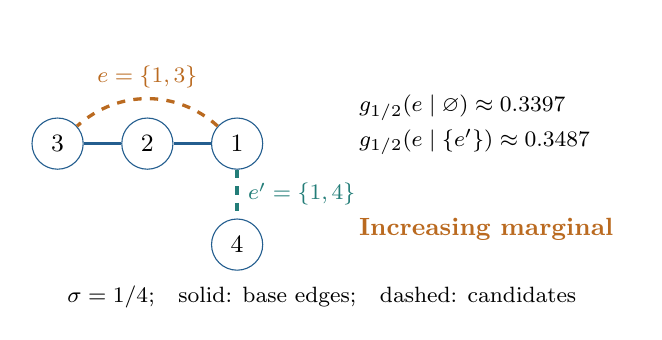
\begin{tikzpicture}[x=.95cm,y=.95cm,
vtx/.style={circle,draw=PolarBlue,fill=white,minimum size=6.5mm,inner sep=0pt,font=\small},
every node/.style={font=\footnotesize}]
\path[use as bounding box](-.4,-2.25) rectangle(7.7,1.55);
\node[vtx](v3) at(0,0){3};
\node[vtx](v2) at(1.2,0){2};
\node[vtx](v1) at(2.4,0){1};
\node[vtx](v4) at(2.4,-1.35){4};
\draw[line width=1.1pt,PolarBlue](v3)--(v2)--(v1);
\draw[dashed,line width=1.2pt,PolarOrange]
(v1) to[bend right=42] node[above,text=PolarOrange]{$e=\{1,3\}$}(v3);
\draw[dashed,line width=1.2pt,PolarTeal]
(v1)--node[right,text=PolarTeal]{$e'=\{1,4\}$}(v4);
\node[anchor=west,align=left] at(3.9,.25)
{$g_{1/2}(e\mid\varnothing)\approx0.3397$\\[3pt]
 $g_{1/2}(e\mid\{e'\})\approx0.3487$};
\node[anchor=west,text=PolarOrange,font=\bfseries\small] at(3.9,-1.15)
{Increasing marginal};
\node[anchor=west] at(0,-2.05)
{$\sigma=1/4$;\quad solid: base edges;\quad dashed: candidates};
\end{tikzpicture}
\caption{A four-vertex counterexample (Example~\ref{ex:four-vertex}).}
\end{subfigure}\hfill
\begin{subfigure}[t]{.50\textwidth}
\centering
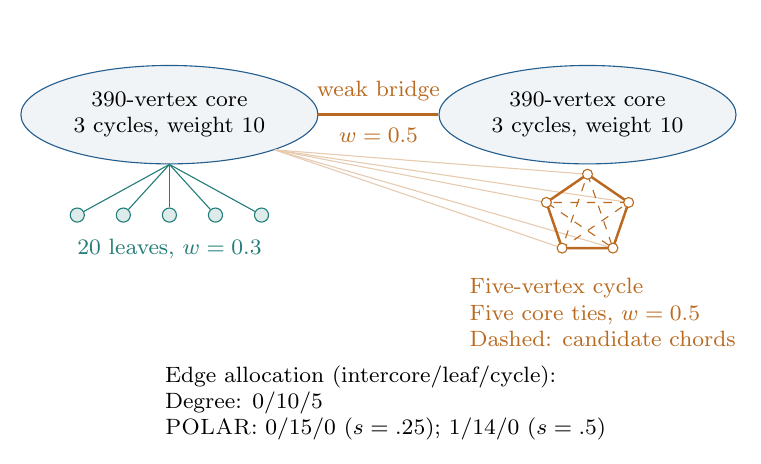
\begin{tikzpicture}[x=.9cm,y=.85cm,every node/.style={font=\footnotesize}]
\path[use as bounding box](-1.1,-4.45) rectangle(8.85,1.65);
\node[ellipse,draw=PolarBlue,fill=PolarBlue!7,
minimum width=2.4cm,minimum height=1.25cm,align=center](left)at(.9,.35)
{390-vertex core\\3 cycles, weight 10};
\node[ellipse,draw=PolarBlue,fill=PolarBlue!7,
minimum width=2.4cm,minimum height=1.25cm,align=center](right)at(6.8,.35)
{390-vertex core\\3 cycles, weight 10};
\draw[line width=1.1pt,PolarOrange](left.east)--
node[above=1pt]{weak bridge} node[below=1pt]{$w=0.5$}(right.west);
\foreach \x [count=\i] in {-.4,.25,.9,1.55,2.2}{
\node[circle,draw=PolarTeal,fill=PolarTeal!15,inner sep=1.8pt](leaf\i)at(\x,-1.15){};
\draw[PolarTeal,thin](left.south)--(leaf\i);
}
\node[text=PolarTeal]at(.9,-1.65){20 leaves, $w=0.3$};
\foreach \i/\ang in {0/90,1/18,2/-54,3/-126,4/162}{
  \coordinate (c\i) at ($(6.8,-1.15)+(\ang:.61)$);
  \draw[PolarOrange!35,thin](left.south east)--(c\i);
}
\draw[PolarOrange,line width=.9pt](c0)--(c1)--(c2)--(c3)--(c4)--cycle;
\draw[PolarOrange,dashed,thin](c0)--(c2)--(c4)--(c1)--(c3)--cycle;
\foreach \i in {0,1,2,3,4}{
  \filldraw[draw=PolarOrange,fill=white](c\i)circle(1.8pt);
}
\node[anchor=north west,align=left,text=PolarOrange]at(5.0,-1.95)
{Five-vertex cycle\\Five core ties, $w=0.5$\\Dashed: candidate chords};
\node[anchor=north,align=left]at(3.95,-3.25)
{Edge allocation (intercore/leaf/cycle):\\
 Degree: $0/10/5$\\
 \POLAR{}: $0/15/0$ ($s=.25$); $1/14/0$ ($s=.5$)};
\end{tikzpicture}
\caption{Controlled multiscale graph ($n=805$).}
\end{subfigure}
\caption{Two aspects of fractional spectral link selection.
(a) A four-vertex violation of diminishing returns: inserting $e'$
increases the marginal gain of $e$. Solid edges belong to the base
graph; dashed edges are candidates. (b) Schematic of the controlled
multiscale benchmark ($n=805$), comprising two dense cores, a weak
bridge, peripheral leaves, and a locally anchored cycle. Five of
the twenty leaves are illustrated. Edge allocations and fractional
gains are reported in Table~\ref{tab:multiscale}.}
\label{fig:motivation}
\end{figure*}
To quantify what a candidate contributes, interpolate between
$\matA_S$ and its single-edge update. For $e\in\mathcal C\setminus S$,
let $\matA_u=\matA_S+u b_eb_e^\top$ for $0\le u\le1$. Here $u$ is
an edge-insertion parameter. Let $\lambda_i(u)$ and $v_i(u)$,
for $1\le i\le n$, be eigenvalues and orthonormal eigenvectors
of $L_S+u b_eb_e^\top$. Thus $\matA_u$ has eigenvalues
$\lambda_i(u)+\sigma$. The following identity measures the
full marginal by sensitivity along this update path.
\begin{lemma}[Spectral sensitivity]
\label{lem:spectral-sensitivity}
For every $0<s<1$,
\begin{equation}
\begin{aligned}
g_s(e\mid S)
&=s\int_0^1 b_e^\top \matA_u^{-s-1}b_e\,du\\
&=\int_0^1\sum_{i=1}^n
\frac{s(v_i(u)^\top b_e)^2}{(\lambda_i(u)+\sigma)^{s+1}}\,du.
\end{aligned}
\label{eq:path-marginal}
\end{equation}
In particular, every candidate has a strictly positive marginal.
\end{lemma}
\begin{proof}
Set $c_s=\sin(\pi s)/\pi>0$. The Stieltjes identity, derived explicitly in~\eqref{eq:stieltjes}, gives
\[
\Tr({\matA}_u^{-s})
=c_s\int_0^\infty t^{-s}\Tr(({\matA}_u+t I)^{-1})\,dt,
\]
Differentiating an inverse and using cyclic invariance of trace gives
\[
\frac{d}{du}\Tr(({\matA}_u+t I)^{-1})
=-b_e^\top({\matA}_u+t I)^{-2}b_e.
\]
The absolute value is at most $2/(\sigma+t)^2$. Its product with $t^{-s}$ is integrable at zero because $s<1$ and at infinity because $s>0$. Differentiation under the integral is therefore valid. Differentiating the scalar Stieltjes identity and applying it to each eigenvalue of ${\matA}_u$ yields
\[
\begin{aligned}
-\frac{d}{du}\Tr({\matA}_u^{-s})
&=c_s\int_0^\infty{ t}^{-s}b_e^\top({\matA}_u+t I)^{-2}b_e\,dt\\
&=s b_e^\top {\matA}_u^{-s-1}b_e.
\end{aligned}
\]
Integrating from zero to one proves the first equality in~\eqref{eq:path-marginal}. Diagonalizing ${\matA}_u$ proves the second. The quadratic form is positive because ${\matA}_u^{-s-1}\succ0$ and $b_e\ne0$, proving strict positivity.
\end{proof}
For a simple eigenvalue, $\dot\lambda_i(u)=(v_i(u)^\top b_e)^2$,
where the dot denotes differentiation along the insertion path.
Its sensitivity weight is $w_s(\lambda)=s(\lambda+\sigma)^{-s-1}$.
Smaller $s$ reduces the relative dominance of low-frequency modes,
a preference that also has a diffusion-time interpretation.

\paragraph*{Diffusion time scales}
For diffusion time $\tau>0$ and a Laplacian $L$,
the heat trace $\Tr(e^{-\tau L})$ is the sum of continuous-time
random-walk return probabilities. Let
$\Delta\mathcal H_S(\tau)=\Tr(e^{-\tau L_0})-\Tr(e^{-\tau L_S})\ge0$
denote its reduction after inserting $S$, and let $\Gamma(s)$
be the Gamma function. For the short-time expansion, define
$\Delta_S\Tr(L^2)=\Tr(L_S^2)-\Tr(L_0^2)$.
When inserting a candidate edge $\{u,v\}$, let $d_u,d_v$
denote its endpoints' current weighted degrees. We write
$w_{uv}$ for the current edge weight between $u$ and $v$
(zero if absent).

\begin{proposition}[Heat-trace representation]
\label{prop:heat}
For $0<s<1$,
\begin{align}
f_s(S)&=\frac1{\Gamma(s)}\int_0^\infty \tau^{s-1}e^{-\sigma \tau}
\Delta\mathcal H_S(\tau)\,d\tau,\label{eq:heat-mellin}\\
f_{\log}(S)&=\int_0^\infty \tau^{-1}e^{-\sigma \tau}\Delta\mathcal H_S(\tau)\,d\tau,
\notag
\end{align}
and the same formula with $s=1$ gives the inverse-trace gain.
As $\tau\to0$,
$\Delta\mathcal H_S(\tau)=2|S|\tau-\frac{\tau^2}{2}\Delta_S\Tr(L^2)+O(\tau^3)$,
where adding $\{u,v\}$ increases $\Tr(L^2)$ by $2(d_u+d_v)+4$.
\end{proposition}
\begin{proof}
The fractional-power and logarithmic integral representations
applied to the eigenvalues of $\matA_0$ and $\matA_S$, together with
$\Tr(e^{-\tau \matA})=e^{-\sigma \tau}\Tr(e^{-\tau L})$ for
$\matA=L+\sigma I$, give the stated formulas.
Monotonicity of the heat trace under Laplacian addition gives
$\Delta\mathcal H_S(\tau)\ge0$. Expanding the exponential and using
$\Tr(L^2)=\sum_vd_v^2+\sum_{u\ne v}w_{uv}^2$ yields the short-time terms.
\end{proof}

The kernel in~\eqref{eq:heat-mellin} is proportional to a Gamma
density with shape $s$, rate $\sigma$, and mean $s/\sigma$;
consequently, $f_s$ equals $\sigma^{-s}$ times the corresponding
expected heat-trace reduction. At fixed budget, selections share the leading short-time term;
the next term favors smaller endpoint-degree sums. Increasing $s$
emphasizes longer times, whereas increasing $\sigma$ emphasizes
shorter times.

Changing $s$ can reverse edge rankings even as $\sigma\to0^+$.
When an insertion does not merge components, the zero-mode
contributions cancel, leaving the difference of
$\sum_{\lambda>0}\lambda^{-s}$ over the nonzero Laplacian
eigenvalues. Consider a unit-weight triangle on $\{1,2,3\}$,
with leaves $4,5$ attached to vertex $1$ and leaf $6$ attached
to vertex $2$. In the $\sigma\to0^+$ limit, inserting $\{4,5\}$
or $\{2,4\}$ yields gains of $0.423$ and $0.403$ at $s=1/2$,
but $2/3$ and $13/18$ at $s=1$, respectively. Their ranking
therefore reverses. Indeed, the Laplacian characteristic polynomials of the base graph
and of the graphs with $\{2,4\}$ and $\{4,5\}$ added are
$x(x-1)Q(x)$, $x(x-2)(x^2-6x+4)(x^2-6x+6)$, and $x(x-3)Q(x)$, with
$Q(x)=x^4-11x^3+39x^2-49x+18$. Hence $\{4,5\}$ gains $1-3^{-s}$
(it is a twin pair, cf.\ Proposition~\ref{prop:twins}), the
pseudoinverse traces are $67/18$, $3$, and $55/18$, and the $s=\frac12$
gain of $\{2,4\}$ is $0.4025436208$. Both strict orders persist for all
sufficiently small $\sigma>0$ by continuity. A link that joins two
components instead adds $\sigma^{-s}+O(1)$ for every $s$, so with a
candidate pool spanning components all exponents first favor merging
links as $\sigma\to0$.


\subsection{An Exact Obstruction to Submodularity}
Strictly positive marginals need not exhibit diminishing
returns. For selected-edge sets $A\subseteq T\subseteq\mathcal C$,
submodularity would require $g_s(e\mid A)\ge g_s(e\mid T)$
for any remaining edge $e\in\mathcal C\setminus T$: inserting other edges could
never increase the value of a remaining edge. The following
exact example violates this condition.

\begin{example}[A four-vertex obstruction to submodularity]
\label{ex:four-vertex}
Let $V=\{1,2,3,4\}$, $E_0=\{\{1,2\},\{2,3\}\}$, $\sigma=1/4$, and $s=1/2$.
All base and added edges have unit weight. Let $e=\{1,3\}$ and $e'=\{1,4\}$.
For the normalized gain $f_s$, its marginals obey
\begin{align}
 g_s(e\mid\varnothing)&=\frac{2}{\sqrt5}-\frac{2}{\sqrt{13}},\\
 g_s(e\mid\{e'\})&=\frac{8\sqrt2}{7}+\frac23
 -\frac2{\sqrt5}-\frac2{\sqrt{13}}-\frac2{\sqrt{17}},
\end{align}
and $g_s(e\mid\{e'\})-g_s(e\mid\varnothing)>1/375>0$.
Thus $f_s$ is not submodular, even for unweighted base graphs and unit-weight additions.
\end{example}
\begin{proof}
The base graph is a three-vertex path and an isolated vertex, so its Laplacian has eigenvalues $0,0,1,3$.
Indeed, $(1,1,1,0)^\top$ and $(0,0,0,1)^\top$ are zero eigenvectors, while $(1,0,-1,0)^\top$ and $(1,-2,1,0)^\top$ have eigenvalues $1$ and $3$.
Adding $e$ gives a triangle and an isolated vertex, with eigenvalues $0,0,3,3$: every vector supported on the first three coordinates and summing to zero has eigenvalue $3$.

Adding ${e'}$ to the base graph gives the path $3$--$2$--$1$--$4$, whose Laplacian is
\[
L_{e'}=\begin{pmatrix}
2&-1&0&-1\\-1&2&-1&0\\0&-1&1&0\\-1&0&0&1
\end{pmatrix}.
\]
The subspaces $\{(x,x,y,y)^\top\}$ and $\{(x,-x,y,-y)^\top\}$ are invariant.
On these subspaces, the coordinate matrices are respectively
$\bigl(\begin{smallmatrix}1&-1\\-1&1\end{smallmatrix}\bigr)$ and
$\bigl(\begin{smallmatrix}3&1\\1&1\end{smallmatrix}\bigr)$.
Their eigenvalues are $0,2$ and $2-\sqrt2,2+\sqrt2$, respectively.
After adding both edges, the graph is a triangle with a pendant vertex.
Its eigenvectors $(1,1,1,1)^\top$, $(0,1,1,-2)^\top$,
$(0,1,-1,0)^\top$, and $(-3,1,1,1)^\top$ have eigenvalues $0,1,3,4$.
These four independent vectors give the complete spectrum.

Adding $\sigma I$ shifts every eigenvalue by $1/4$.
Subtracting the trace of the inverse square root after adding $e$ from the trace before adding it therefore gives
$g_s(e\mid\varnothing)=2/\sqrt5-2/\sqrt{13}$.
For the second marginal, the three nonzero path eigenvalues contribute
\[
\frac2{\sqrt{9-4\sqrt2}}+\frac23+
\frac2{\sqrt{9+4\sqrt2}}.
\]
Both terms in the following sum are positive, and
\[
\left(\frac1{\sqrt{9-4\sqrt2}}+
\frac1{\sqrt{9+4\sqrt2}}\right)^2
=\frac{18}{49}+\frac27=\frac{32}{49}.
\]
Consequently the sum equals $4\sqrt2/7$.
The common zero-eigenvalue contribution cancels, yielding the stated second marginal.
Their difference is
\[
D=\frac{8\sqrt2}{7}+\frac23-\frac4{\sqrt5}-\frac2{\sqrt{17}}.
\]
The inequalities $707^2<2\cdot500^2$, $16\cdot10000<5\cdot179^2$,
and $4\cdot10000<17\cdot49^2$ imply
\[
\sqrt2>\frac{707}{500},\qquad
\frac4{\sqrt5}<\frac{179}{100},\qquad
\frac2{\sqrt{17}}<\frac{49}{100}.
\]
Substitution gives
\[
D>\frac87\frac{707}{500}+\frac23
-\frac{179}{100}-\frac{49}{100}=\frac1{375}>0.
\]
This strictly reverses the diminishing-returns inequality for
$\varnothing\subset\{{e'}\}$ and $e\notin\{{e'}\}$.
\end{proof}

Numerically, the two marginals are $0.3397269948$ and $0.3487121007$; the strict inequality above is certified without floating-point arithmetic.

Hence stale marginal values cannot serve as valid lazy upper bounds;
Sections~\ref{sec:guarantees} and~\ref{sec:framework} provide
non-submodular guarantees and safe proxy screening instead.

\section{Quadrature-Based Marginal Formula and Approximation Guarantees}
\label{sec:guarantees}

We derive a relative-error marginal oracle and non-submodular greedy
bounds, then combine quadrature, proxy, and solve errors.
This extended version gives complete proofs of all statements.

\subsection{Positive Composite Quadrature}
To avoid subtracting two approximate traces, we approximate each
rank-one marginal through a positive Stieltjes representation.
For $0<s<1$, set $c_s=\sin(\pi s)/\pi$; the inverse power
satisfies the following identity for $x>0$.
\begin{equation}
x^{-s}=c_s\int_0^\infty\frac{t^{-s}}{x+t}\,dt.
\label{eq:stieltjes}
\end{equation}
For a spectral interval $[\lambda_{\rm lo},\lambda_{\rm hi}]$ with $0<\lambda_{\rm lo}\le \lambda_{\rm hi}$, set
$K=\lceil\log_2(\lambda_{\rm hi}/\lambda_{\rm lo})\rceil$, $C=2^K\lambda_{\rm lo}$, and $L_\ell=2^\ell \lambda_{\rm lo}$.
Partition the integral into $[0,\lambda_{\rm lo}]$, $K$ middle intervals
$[L_\ell,2L_\ell]$, and $[C,\infty)$. Apply order-$r$
Gauss--Jacobi rules with node--weight pairs $(\ell_i,A_i)$,
$(\xi_i,W_i)$, and $(v_i,B_i)$ for the measures $u^{-s}du$
on $[0,1]$, $du$ on $[-1,1]$, and $u^{s-1}du$ on $[0,1]$,
respectively~\cite{dlmf-quadrature,dlmf-jacobi}. The low, middle,
and transformed high panels give the following positive poles and weights.
\begin{equation}
\begin{alignedat}{2}
t_i^{\mathrm{lo}}&=\lambda_{\rm lo}\ell_i,&\quad
\omega_i^{\mathrm{lo}}&=c_s\lambda_{\rm lo}^{1-s}A_i,\\
t_{\ell i}^{\mathrm{mid}}&=\tfrac{L_\ell}{2}(3+\xi_i),&
\omega_{\ell i}^{\mathrm{mid}}&=c_s\tfrac{L_\ell}{2}W_i
(t_{\ell i}^{\mathrm{mid}})^{-s},\\
t_i^{\mathrm{hi}}&=C/v_i,&
\omega_i^{\mathrm{hi}}&=c_sC^{1-s}B_i/v_i.
\end{alignedat}
\label{eq:poles}
\end{equation}
Enumerating these poles as $(t_j,\omega_j)_{j=1}^q$ gives
$q=(K+2)r$ positive poles and weights, with neither tail truncated.
Their sum defines the rational approximation below.
\begin{equation}
r_q(x)=\sum_{j=1}^q\frac{\omega_j}{x+t_j}.
\label{eq:rational}
\end{equation}

\subsection{Dimension-Free Relative Marginal Error}
By Lemma~\ref{lem:spectral-sensitivity}, relative approximation
of the positive derivative controls the marginal without subtracting
approximate traces. Gaussian exactness provides this bound panelwise.

\begin{lemma}[A positive Gaussian quadrature estimate]
\label{lem:gaussian-relative}
Let $\mu$ be a finite positive measure on $[-1,1]$ and let $Q_r$ be a positive $r$-point Gaussian rule for $\mu$. Suppose that $F$ is analytic in a neighborhood of $\{z:|z|\le2\}$, that $|F(z)|\le {M_*}$ on $|z|=2$, and that $F(u)\ge {m_*}>0$ on $[-1,1]$. Then
\begin{equation}
\left|\int F\,d\mu-Q_r[F]\right|
\le\frac{4{M_*}}{{m_*}}4^{-r}\int F\,d\mu.
\label{eq:gaussian-relative}
\end{equation}
Moreover, for $\ell(u)=(1+u)/2$, provided $\int\ell\,d\mu>0$,
\begin{equation}
\left|\int\ell F\,d\mu-Q_r[\ell F]\right|
\le\frac{8{M_*}}{{m_*}}4^{-r}\int\ell F\,d\mu.
\label{eq:gaussian-linear-relative}
\end{equation}
\end{lemma}
\begin{proof}
Write the Taylor series $F(z)=\sum_{\nu=0}^\infty a_\nu z^\nu$. Cauchy's coefficient estimate on $|z|=2$ gives $|a_\nu|\le {M_*}2^{-\nu}$. For $P(u)=\sum_{\nu=0}^{2r-1}a_\nu u^\nu$ and $u\in[-1,1]$,
\[
|F(u)-P(u)|\le {M_*}\sum_{\nu=2r}^\infty2^{-\nu}
=2{M_*}4^{-r}.
\]
Exactness on $P$ and on constants, together with positivity of the weights, yields
\begin{align*}
\left|\int F\,d\mu-Q_r[F]\right|
&=\left|\int(F-P)\,d\mu-Q_r[F-P]\right|\\
&\le2{M_*}4^{-r}\bigl(\mu([-1,1])+Q_r[1]\bigr)\\
&=4{M_*}4^{-r}\mu([-1,1]).
\end{align*}
Since $\int F\,d\mu\ge {m_*}\mu([-1,1])$, this proves \eqref{eq:gaussian-relative}.

For the second assertion, let $P_-(u)=\sum_{\nu=0}^{2r-2}a_\nu u^\nu$. Then
\[
\sup_{[-1,1]}|F-P_-|
\le {M_*}\sum_{\nu=2r-1}^\infty2^{-\nu}=4{M_*}4^{-r}.
\]
The polynomial $\ell P_-$ has degree at most $2r-1$. Since $\ell\ge0$ and $Q_r[\ell]=\int\ell\,d\mu$, we obtain
\begin{align*}
\left|\int\ell F\,d\mu-Q_r[\ell F]\right|
&\le4{M_*}4^{-r}\left(\int\ell\,d\mu+Q_r[\ell]\right)\\
&=8{M_*}4^{-r}\int\ell\,d\mu\\
&\le\frac{8{M_*}}{{m_*}}4^{-r}\int\ell F\,d\mu.
\end{align*}
This is \eqref{eq:gaussian-linear-relative}.
\end{proof}

\begin{lemma}[Uniform relative derivative approximation]
\label{lem:derivative-quadrature}
For \eqref{eq:rational}, define
\[
D(x)=sx^{-s-1},\qquad D_q(x)=\sum_{j=1}^q\frac{\omega_j}{(x+t_j)^2}.
\]
For every $x\in[\lambda_{\rm lo},\lambda_{\rm hi}]$,
\begin{equation}
|D_q(x)-D(x)|\le256\,4^{-r}D(x).
\label{eq:derivative-relative}
\end{equation}
\end{lemma}
\begin{proof}
Differentiating \eqref{eq:stieltjes} under the integral gives
\begin{equation}
D(x)=c_s\int_0^\infty\frac{t^{-s}}{(x+t)^2}\,dt.
\label{eq:derivative-integral}
\end{equation}
The integrable function $t^{-s}/({\lambda_{\rm lo}}+t)^2$ justifies this differentiation uniformly for $x\in[\lambda_{\rm lo},\lambda_{\rm hi}]$. We bound the relative error separately on each positive integral piece.

For the low tail, put $t={\lambda_{\rm lo}}u$ and $v=2u-1$. Apart from the positive factor $c_s{\lambda_{\rm lo}}^{1-s}(x+{\lambda_{\rm lo}}/2)^{-2}$, the kernel against $u^{-s}\,du$ is
\[
F_{\mathrm{lo}}(v)=(1+\theta v)^{-2},\qquad
\theta=\frac {\lambda_{\rm lo}}{2x+{\lambda_{\rm lo}}}\le\frac13.
\]
On $|z|\le2$, $|1+\theta z|\ge1-2\theta\ge1/3$, so the kernel is analytic on a neighborhood of this disk and has boundary modulus at most $9$. For real $v\in[-1,1]$,
\[
F_{\mathrm{lo}}(v)\ge(1+\theta)^{-2}\ge\frac9{16}.
\]
Equation \eqref{eq:gaussian-relative}, applied to the affine image of the measure $u^{-s}\,du$, therefore gives the low-tail relative error $64\,4^{-r}$.

On a middle panel $[L,2L]$, substitute $t=L(3+v)/2$. The positive prefactor is
\[
c_s\frac L2\left(\frac{3L}{2}\right)^{-s}
\left(x+\frac{3L}{2}\right)^{-2},
\]
and the remaining kernel is
\[
F_{\mathrm{mid}}(v)=(1+v/3)^{-s}(1+\theta v)^{-2},
\quad\theta=\frac L{2x+3L}\le\frac13.
\]
The branch positive on the real interval is analytic on $|z|\le2$, because $\operatorname{Re}(1+z/3)\ge1/3$. On its boundary,
\[
|F_{\mathrm{mid}}(z)|\le3^s3^2\le27,
\]
whereas on the real interval,
\[
F_{\mathrm{mid}}(v)\ge(4/3)^{-s-2}\ge\frac{27}{64}.
\]
Equation \eqref{eq:gaussian-relative} gives relative error at most $256\,4^{-r}$ on every middle panel.

For the high tail, the substitution $t=C/u$ gives
\[
c_s\int_C^\infty\frac{t^{-s}}{(x+t)^2}\,dt
=c_sC^{1-s}\int_0^1\frac{u^s}{(C+xu)^2}\,du.
\]
The Gaussian rule in \eqref{eq:poles} is for $u^{s-1}\,du$. Its derivative integrand therefore contains an additional factor $u$. With $v=2u-1$, the kernel, apart from $(C+x/2)^{-2}$, is
\[
\ell(v)F_{\mathrm{hi}}(v),\quad
\ell(v)=\frac{1+v}{2},\quad
F_{\mathrm{hi}}(v)=(1+\theta v)^{-2},
\]
where $\theta=x/(2C+x)\le1/3$, since $x\le\lambda_{\rm hi}\le C$. The same bounds ${M_*}=9$ and ${m_*}=9/16$ hold. Equation \eqref{eq:gaussian-linear-relative} gives the high-tail relative error $128\,4^{-r}$. This rule is precisely the high-tail contribution to $D_q$, because
\[
\frac{\omega_i^{\mathrm{hi}}}{(x+t_i^{\mathrm{hi}})^2}
=c_sC^{1-s}B_i\frac{v_i}{(C+xv_i)^2}.
\]

Let $I_\nu(x)>0$ be the exact derivative contribution of a panel, and let $\widetilde I_\nu(x)$ be its quadrature. Each preceding bound is at most $256\,4^{-r}I_\nu(x)$. Thus
\begin{align*}
|D_q(x)-D(x)|
&\le\sum_\nu|\widetilde I_\nu(x)-I_\nu(x)|\\
&\le256\,4^{-r}\sum_\nu I_\nu(x)
=256\,4^{-r}D(x).
\end{align*}
Positivity prevents a factor proportional to the number of panels from appearing.
\end{proof}

Spectral calculus extends the derivative bound to
$\matA+u b_eb_e^\top$, $0\le u\le1$, whenever its
spectrum lies in $[\lambda_{\rm lo},\lambda_{\rm hi}]$. Integration then gives
a dimension-free relative marginal guarantee.

\begin{theorem}[Dimension-free relative marginal approximation]
\label{thm:dimension-free-marginal}
Let $\matA\succ0$ and $b_e\ne0$, and suppose that
\[
\operatorname{spec}(\matA+u b_eb_e^\top)\subseteq[\lambda_{\rm lo},\lambda_{\rm hi}]
\quad\text{for every }u\in[0,1].
\]
Let $0<s<1$ and $0<\epsilon\le1/2$. Construct \eqref{eq:rational} with $r=\lceil\log_4(256/\epsilon)\rceil$. All weights and poles are positive, and
\[
q=\bigl(\lceil\log_2(\lambda_{\rm hi}/\lambda_{\rm lo})\rceil+2\bigr)r
=O\bigl((1+\log(\lambda_{\rm hi}/\lambda_{\rm lo}))\log(1/\epsilon)\bigr).
\]
The rational marginal is
\begin{equation}
\widetilde\Delta_s(e;\matA)
=-\sum_{j=1}^q\omega_j
\frac{b_e^\top(\matA+t_jI)^{-2}b_e}
{1+b_e^\top(\matA+t_jI)^{-1}b_e}.
\label{eq:multi-pole-marginal}
\end{equation}
For $\Delta_s(e;\matA)=\Tr((\matA+b_eb_e^\top)^{-s})-\Tr(\matA^{-s})$, it satisfies
\begin{equation}
|\widetilde\Delta_s(e;\matA)-\Delta_s(e;\matA)|
\le\epsilon|\Delta_s(e;\matA)|.
\label{eq:dimension-free-marginal}
\end{equation}
\end{theorem}
\begin{proof}
Equation \eqref{eq:poles} gives positive weights and poles, numbering $(K+2)r$, which proves the pole-count assertion.

Write $R_j=({\matA}+t_jI)^{-1}$. Its positive definiteness implies $1+b_e^\top R_jb_e>0$. The Sherman--Morrison identity gives
\[
({\matA}+t_jI+b_eb_e^\top)^{-1}
=R_j-\frac{R_jb_eb_e^\top R_j}{1+b_e^\top R_jb_e}.
\]
Taking traces and using their cyclic invariance yields
\[
\Tr\bigl(({\matA}+t_jI+b_eb_e^\top)^{-1}-R_j\bigr)
=-\frac{b_e^\top R_j^2b_e}{1+b_e^\top R_jb_e}.
\]
Multiplication by $\omega_j$ and summation proves \eqref{eq:multi-pole-marginal}; it is exactly the trace difference of $r_q$.

Set ${\matA}_u={\matA}+u b_eb_e^\top$. Differentiating the resolvent gives
\[
\frac{d}{du}({\matA}_u+t I)^{-1}
=-({\matA}_u+t I)^{-1}b_eb_e^\top({\matA}_u+t I)^{-1}.
\]
The absolute value of its trace is at most $\|b_e\|^2/({\lambda_{\rm lo}}+t)^2$. Since $\int_0^\infty{ t}^{-s}/({\lambda_{\rm lo}}+t)^2\,dt$ is finite, differentiation under the trace Stieltjes integral is justified. Consequently,
\begin{align*}
\frac{d}{du}\Tr({\matA}_u^{-s})
&=-c_s\int_0^\infty{ t}^{-s}
b_e^\top({\matA}_u+t I)^{-2}b_e\,dt\\
&=-b_e^\top D({\matA}_u)b_e.
\end{align*}
The last equality follows by applying \eqref{eq:derivative-integral} to each eigenvalue of ${\matA}_u$. Differentiating the finite rational sum similarly gives
\[
\frac{d}{du}\Tr(r_q({\matA}_u))=-b_e^\top D_q({\matA}_u)b_e.
\]
The fundamental theorem of calculus now yields
\[
-\Delta_s(e;{\matA})=\int_0^1b_e^\top D({\matA}_u)b_e\,du,
\]
and
\[
-\widetilde\Delta_s(e;{\matA})=\int_0^1b_e^\top D_q({\matA}_u)b_e\,du.
\]

Lemma~\ref{lem:derivative-quadrature} and the chosen $r$ imply
\[
(1-\epsilon)D(x)\le D_q(x)\le(1+\epsilon)D(x)
\quad(x\in[\lambda_{\rm lo},\lambda_{\rm hi}]).
\]
Diagonalize ${\matA}_u=V_u\Lambda_uV_u^\top$. Both $D({\matA}_u)$ and $D_q({\matA}_u)$ use this same eigenbasis, and every eigenvalue belongs to $[\lambda_{\rm lo},\lambda_{\rm hi}]$. Applying the scalar inequalities to each diagonal entry therefore proves
\[
(1-\epsilon)D({\matA}_u)\preceq D_q({\matA}_u)
\preceq(1+\epsilon)D({\matA}_u).
\]
Taking quadratic forms with $b_e$ and integrating gives
\[
(1-\epsilon)(-\Delta_s(e;{\matA}))
\le-\widetilde\Delta_s(e;{\matA})
\le(1+\epsilon)(-\Delta_s(e;{\matA})).
\]
Since $D({\matA}_u)=s{\matA}_u^{-s-1}\succ0$ and $b_e\ne0$, the quantity $-\Delta_s(e;{\matA})$ is positive. Rearranging proves \eqref{eq:dimension-free-marginal}.
\end{proof}

By~\eqref{eq:spectral-window}, $\lambda_{\rm lo}=\sigma$ and $\lambda_{\rm hi}=\Lambda$
cover all relevant update paths of at most $2k$ edges.

For algebraic evaluation at state $S$, set
$u_j=(\matA_S+t_jI)^{-1}b_e$. By symmetry, the positive
rational marginal is
\[
G_q(e\mid S)=-\widetilde\Delta_s(e;\matA_S)
=\sum_{j=1}^q\omega_j\frac{\|u_j\|_2^2}{1+b_e^\top u_j}.
\]
Theorem~\ref{thm:dimension-free-marginal} controls $G_q$ without
projection error. To avoid evaluating every candidate algebraically,
\POLAR{} uses a proxy shortlist (Section~\ref{sec:framework}).


\subsection{The Log-Determinant Reference Objective}
\begin{proposition}[Strict monotonicity and submodularity of log-determinant gain]
\label{prop:logdet-submodularity}
For the normalized log-determinant gain $f_{\log}$, every nonzero
edge addition has positive marginal gain, and $f_{\log}$ is
submodular. For two distinct candidates, diminishing returns is
strict exactly when their inverse-matrix cross term is nonzero.
\end{proposition}
\begin{proof}
Fix $S$ and an unselected edge $e$, and write $R=\matA_{S}^{-1}$.
The matrix determinant lemma gives
\[
g_{\log}(e\mid S)=\log(1+b_e^\top Rb_e)>0,
\]
because $R$ is positive definite and $b_e\ne0$.
For $S\subseteq T$, let $A=\matA_{S}$ and $H=\matA_{T}-\matA_{S}\succeq0$.
Writing $C=A^{-1/2}HA^{-1/2}\succeq0$ gives
\[
\matA_{T}^{-1}=A^{-1/2}(I+C)^{-1}A^{-1/2}\preceq A^{-1},
\]
since every eigenvalue of $(I+C)^{-1}$ is at most one.
Thus $b_e^\top \matA_{T}^{-1}b_e\le b_e^\top \matA_{S}^{-1}b_e$;
applying the increasing function $x\mapsto\log(1+x)$ proves diminishing returns.

More explicitly, for distinct unselected edges $e,{e'}$, put
$d_e=b_e^\top Rb_e$, $d_{e'}=b_{e'}^\top Rb_{e'}$, and $c=b_e^\top Rb_{e'}$.
Sherman--Morrison gives
\[
\begin{aligned}
&g_{\log}(e\mid S\cup\{{e'}\})-g_{\log}(e\mid S)\\
&\qquad=\log\left(1-\frac{c^2}{(1+d_e)(1+d_{e'})}\right)\le0.
\end{aligned}
\]
The logarithm is well-defined because Cauchy--Schwarz in the $R$-inner product yields
$c^2\le d_ed_{e'}<(1+d_e)(1+d_{e'})$.
The inequality is strict exactly when $c\ne0$.

For a connected equality example, take the unweighted four-cycle
$E_0=\{12,23,34,14\}$ and its two missing diagonals $e=13$ and ${e'}=24$.
Their incidence vectors are orthogonal eigenvectors of $L_0$, both with eigenvalue $2$.
Hence $Rb_{e'}=b_{e'}/(\sigma+2)$ and $b_e^\top Rb_{e'}=0$.
The preceding equality shows that adding one diagonal does not change the log-determinant marginal of the other.
\end{proof}

\subsection{Submodularity Ratio and Budget-Restricted Curvature}
For disjoint $S,T\subseteq\mathcal C$, write
$g_s(T\mid S)=f_s(S\cup T)-f_s(S)$. At budget $k\ge1$,
the restricted submodularity ratio compares individual and joint gains:
\begin{equation}
 \gamma_k=
 \inf_{\substack{S\cap T=\varnothing,\ |S|\leq k-1\\
                  1\leq |T|\leq k}}
 \frac{\sum_{e\in T}g_s(e\mid S)}{g_s(T\mid S)}.
 \label{eq:restricted-gamma}
\end{equation}
Restricted generalized curvature measures marginal deterioration
across nested states:
\begin{equation}
 \alpha_{2k}=1-
 \inf_{\substack{A\subseteq T,\ e\notin T\\ |T|+1\leq2k}}
 \frac{g_s(e\mid T)}{g_s(e\mid A)}.
 \label{eq:restricted-alpha}
\end{equation}
All sets are subsets of $\mathcal C$; Lemma~\ref{lem:spectral-sensitivity}
ensures positive denominators. Singleton $T$ and $A=T$ give
$\gamma_k\le1$ and $\alpha_{2k}\ge0$. The $2k$ restriction
covers greedy--optimal unions.

\begin{theorem}[Submodularity ratio and curvature]
\label{thm:ratio-curvature}
Let $0<s<1$, $\sigma>0$, and unit-weight candidate edges with
$\|b_e\|_2^2=2$. With $\Lambda$ defined in~\eqref{eq:spectral-window},
$f_s$ is normalized and strictly increasing, and the following
bounds hold:
\begin{align}
 \gamma_k&\geq\gamma_0
 :=\frac{\sigma}{2s}
       \left[1-\left(\frac{\sigma}{\sigma+2}\right)^s\right]>0,
 \label{eq:gamma-zero}\\
 \alpha_{2k}&\leq\alpha_0
 :=1-\left(\frac{\sigma}{\Lambda}\right)^{s+1}<1.
 \label{eq:alpha-zero}
\end{align}
In fact, the bound in \eqref{eq:gamma-zero} holds without a cardinality
restriction on $S$ or $T$.
\end{theorem}
\begin{proof}
Set $c_s=\sin(\pi s)/\pi>0$.  Fix an SPD matrix $A\succeq\sigma I$
and a nonzero unit-edge vector $b$.  For $t>0$, write
$R_t=(A+t I)^{-1}$,
$d_t=b^\top R_t b$, and
${\phi}_t=b^\top R_t^2b$.
The Stieltjes representation and the Sherman--Morrison identity give
\begin{equation}
 \Tr(A^{-s})-\Tr((A+bb^\top)^{-s})
 =c_s\int_0^\infty{ t}^{-s}
                 \frac{{\phi}_t}{1+d_t}\,dt.
 \label{eq:ratio-sm-integral}
\end{equation}
Every integrand is strictly positive.  The integral is finite because
it is $O(t^{-s})$ at zero and $O(t^{-s-2})$ at infinity.
Consequently every candidate has a strictly positive marginal, and
$f_s(\varnothing)=0$ proves normalization and strict monotonicity.

Differentiating the scalar Stieltjes identity under the integral gives
\[
 sx^{-s-1}=c_s\int_0^\infty
                       \frac{t^{-s}}{(x+t)^2}\,dt.
\]
This differentiation is justified locally uniformly for $x>0$ by an
integrable bound of the form $Ct^{-s}$ on $(0,1)$ and
$Ct^{-s-2}$ on $(1,\infty)$.
Applying the resulting identity in an eigenbasis of $A$ yields
\begin{equation}
 D(A,b):=s b^\top A^{-s-1}b
       =c_s\int_0^\infty{ t}^{-s}{\phi}_t\,dt.
 \label{eq:initial-directional-gain}
\end{equation}
Since $d_t\leq\|b\|_2^2/(\sigma+t)=2/(\sigma+t)$,
\begin{equation}
 \Tr(A^{-s})-\Tr((A+bb^\top)^{-s})
 \geq c_s\int_0^\infty{ t}^{-s}{\phi}_t
                       \frac{\sigma+t}{\sigma+t+2}\,dt.
 \label{eq:marginal-lower-weight}
\end{equation}
Let $\mu_i\geq\sigma$ be the eigenvalues of $A$, with orthonormal
eigenvectors $v_i$, and let $z_i=(v_i^\top b)^2\geq0$.
Then ${\phi}_t=\sum_i z_i/(\mu_i+t)^2$.
For $\mu\geq\sigma$, define
\[
 I(\mu)=\int_0^\infty
  \frac{t^{-s}}{(\mu+t)^2}
  \frac{\sigma+t}{\sigma+t+2}\,dt.
\]
The substitution $t=\mu u$ gives
\begin{align}
 I(\mu)
 &=\mu^{-s-1}\int_0^\infty
   \frac{u^{-s}}{(1+u)^2}
   \frac{\sigma+\mu u}{\sigma+\mu u+2}\,du\notag\\
 &\geq\left(\frac{\mu}{\sigma}\right)^{-s-1}I(\sigma).
 \label{eq:scaled-kernel-comparison}
\end{align}
Indeed, $y/(y+2)$ is increasing for $y>0$, and $\mu\geq\sigma$.
At the endpoint $\mu=\sigma$, partial fractions and the Stieltjes
identity imply
\begin{align*}
 c_s I(\sigma)
 &=c_s\int_0^\infty
   \frac{t^{-s}}{(\sigma+t)(\sigma+t+2)}\,dt\\
 &=\frac12\left[\sigma^{-s}-(\sigma+2)^{-s}\right]
 =\gamma_0s\sigma^{-s-1}.
\end{align*}
Substituting this equality into \eqref{eq:scaled-kernel-comparison}
and then into \eqref{eq:marginal-lower-weight} proves
\begin{equation}
 \Tr(A^{-s})-\Tr((A+bb^\top)^{-s})
 \geq\gamma_0s\sum_i z_i\mu_i^{-s-1}
 =\gamma_0D(A,b).
 \label{eq:single-versus-derivative}
\end{equation}

To compare this single-edge inequality with a joint gain, let
$H=\sum_{e\in T}b_eb_e^\top\succeq0$ and
$K_t=R_t^{1/2}HR_t^{1/2}\succeq0$.
Since $x/(1+x)\leq x$ for $x\geq0$, the spectral theorem gives
\[
 0\preceq I-(I+K_t)^{-1}\preceq K_t.
\]
Congruence with $R_t^{1/2}$ therefore gives
\begin{align*}
 R_t-(A+H+t I)^{-1}
 &=R_t^{1/2}[I-(I+K_t)^{-1}]R_t^{1/2}\\
 &\preceq R_t H R_t.
\end{align*}
Taking traces, integrating with positive weight $c_st^{-s}$,
and using \eqref{eq:initial-directional-gain} yields
\begin{equation}
 \Tr(A^{-s})-\Tr((A+H)^{-s})
 \leq\sum_{e\in T}D(A,b_e).
 \label{eq:joint-versus-derivative}
\end{equation}
Apply \eqref{eq:single-versus-derivative} to each $e\in T$ at
$A=\matA_{S}$ and sum.  Combining the result with
\eqref{eq:joint-versus-derivative} proves
$\sum_{e\in T}g_s(e\mid S)\geq\gamma_0g_s(T\mid S)$.
No cardinality restriction was used in this argument.
The identity
\[
 \gamma_0=\int_0^1
              \left(\frac{\sigma}{\sigma+2t}\right)^{s+1}dt
\]
also shows directly that $0<\gamma_0<1$.

It remains to prove the curvature bound.  For every vector $x$,
\begin{align*}
 x^\top L_0x
 &=\sum_{\{u,v\}\in E_0}w_{uv}(x_u-x_v)^2\\
 &\leq2\sum_v d_{v,0}x_v^2
 \leq2d_{\max,0}\|x\|_2^2.
\end{align*}
Each added edge has operator norm
$\|b_eb_e^\top\|_2=2$.  Thus every matrix formed from at most $2k$
added unit edges, including any partially added last edge, has all
eigenvalues in $[\sigma,\Lambda]$.
The resolvent derivative
$\frac{d}{du}(A+ubb^\top+t I)^{-1}
=-(A+ubb^\top+t I)^{-1}bb^\top
  (A+ubb^\top+t I)^{-1}$,
the same integrable bounds as above, and cyclicity of the trace give
\begin{equation}
 g_s(e\mid S)=s\int_0^1
 b_e^\top(\matA_{S}+u b_eb_e^\top)^{-s-1}b_e\,du.
 \label{eq:curvature-path}
\end{equation}
The spectral theorem, applied separately at each $u$, implies
\[
 \Lambda^{-s-1}I\preceq
 (\matA_{S}+u b_eb_e^\top)^{-s-1}
 \preceq\sigma^{-s-1}I.
\]
Hence whenever $|S|+1\leq2k$,
\[
 2s\Lambda^{-s-1}\leq g_s(e\mid S)
                         \leq2s\sigma^{-s-1}.
\]
For every pair $A\subseteq T$ appearing in
\eqref{eq:restricted-alpha}, these bounds give
\[
 \frac{g_s(e\mid T)}{g_s(e\mid A)}
 \geq\left(\frac{\sigma}{\Lambda}\right)^{s+1}.
\]
Taking the infimum proves \eqref{eq:alpha-zero}.
The comparison applies scalar spectral bounds separately to each path matrix.
\end{proof}



\subsection{A Complete Approximate-Greedy Guarantee}

Following~\cite{bian2017}, we analyze approximate
greedy selection with a recovery factor $\beta$.
Let $S_i$ be the set after round $i$, $e_i$ the
selected edge, and $O$ an optimal budget-$k$ set.

\begin{lemma}[Approximate greedy selection]
\label{lem:approximate-greedy}
Let $f_s$ be normalized and monotone, with well-defined parameters
$\gamma_k\ge\gamma>0$ and $\alpha_{2k}\le\alpha\le1$ from
\eqref{eq:restricted-gamma}--\eqref{eq:restricted-alpha}.
Let $S_0=\varnothing$ and $S_i=S_{i-1}\cup\{e_i\}$, where
\begin{equation}
 g_s(e_i\mid S_{i-1})\geq
 \beta\max_{e\in\mathcal C\setminus S_{i-1}}g_s(e\mid S_{i-1}),
 \qquad 0<\beta\leq1.
 \label{eq:beta-greedy-condition}
\end{equation}
For an optimal set $O$ of cardinality at most $k$, put
$\theta=\beta\gamma$ and
\begin{equation}
 \Phi_k(\alpha,\theta)
 :=\frac{\theta}{k}\sum_{\ell=0}^{k-1}
       \left(1-\frac{\alpha\theta}{k}\right)^\ell.
 \label{eq:finite-greedy-bound}
\end{equation}
Then $f_s(S_k)\geq \Phi_k(\alpha,\theta)f_s(O)$.
For $\alpha>0$,
\[
 \Phi_k(\alpha,\theta)
 =\frac{1-(1-\alpha\theta/k)^k}{\alpha}
 \geq\frac{1-e^{-\alpha\theta}}{\alpha};
\]
for $\alpha=0$, $\Phi_k(0,\theta)=\theta$.
\end{lemma}

\begin{proof}
If $f_s(O)=0$ the claim is immediate; otherwise extend $O$ to
size $k$ by monotonicity. Put $\rho_i=g_s(e_i\mid S_{i-1})$,
$x_i=\rho_i/f_s(O)$, and $w_r=|S_r\cap O|$. Adding
$S_r\setminus O$ to $O$ in greedy order and applying curvature,
then using the ratio and approximate-greedy conditions, gives
\[
\begin{aligned}
f_s(O\cup S_r)-f_s(O)&\ge(1-\alpha)\sum_{i\le r:e_i\notin O}\rho_i,\\
f_s(O\cup S_r)-f_s(S_r)&\le(k-w_r)\rho_{r+1}/\theta.
\end{aligned}
\]
Only unions of at most $2k$ edges occur. Combining yields
\[
1\le\alpha\sum_{i\le r:e_i\notin O}x_i+
\sum_{i\le r:e_i\in O}x_i+(k-w_r)x_{r+1}/\theta.
\]
For the scalar relaxation, let $zC_{m,R}$ be the minimum
remaining gain with residual $z\ge0$, $m\le R$ selections,
and $R$ unselected elements of $O$. Set $C_{0,R}=0$.
An inside increment $x=z$ clears the residual, so
$0\le C_{m,R}\le1$. Therefore
$x+C_{\rm next}\max\{z-cx,0\}$, with $C_{\rm next}$ the next-stage
coefficient, is nondecreasing in $x$ for
$c\in\{\alpha,1\}$, and the least admissible increment
$x=\theta z/R$ minimizes either branch. Outside/inside choices
reduce the residual by $\alpha x$/$x$, respectively; only the
latter reduces $R$. Thus
\[
\begin{split}
C_{m,R}=\frac\theta R+\min\bigl\{&
(1-\alpha\theta/R)C_{m-1,R},\\
&(1-\theta/R)C_{m-1,R-1}\bigr\}.
\end{split}
\]
Induction gives $C_{m,R}=(\theta/R)\sum_{j=0}^{m-1}(1-\alpha\theta/R)^j$,
where $0\le\alpha\theta\le1$. The outside branch attains it;
the inside branch is no smaller because, for $0\le j\le m-2$,
\[
\frac{R-\theta}{R-1}(1-\alpha\theta/(R-1))^j\ge(1-\alpha\theta/R)^{j+1}.
\]
The case $R=2$ is immediate; for $R\ge3$ the ratio on the
right to the power term on the left increases with $j$ and is
at most $J(R)/J(R-1)\le1$, where $J(u)=(1-\alpha\theta/u)^{u-1}$.
Indeed, $(\log J)'(u)\le\log(1-\alpha\theta/u)+\alpha\theta/u\le0$ for $u\ge2$.
At $(m,R,z)=(k,k,1)$ this gives $\Phi_k(\alpha,\theta)$;
the geometric sum and $(1-\alpha\theta/k)^k\le e^{-\alpha\theta}$
give the remaining assertions.
\end{proof}

We next relate $\beta$ to the numerical errors
of \POLAR{}'s marginal evaluations.

\subsection{Numerical Errors and Algebraic Re-ranking}
\label{sec:numerical-errors}

Algebraic-score accuracy additionally requires control of solve residuals.

\begin{lemma}[Residual certification of algebraic reranking scores]
\label{lem:residual-score}
Fix a state $S$, a candidate $e$, and positive quadrature weights
$\omega_j$. For each pole, let $A_j=\matA_S+t_jI$,
$u_j=A_j^{-1}b_e$, and $\lambda_{\rm lo,j}I\preceq A_j\preceq \lambda_{\rm hi,j}I$,
with $\lambda_{\rm lo,j}=\sigma+t_j$ and $\lambda_{\rm hi,j}=\Lambda+t_j$.
For some $0<\rho<1$, suppose the computed solution
$\widetilde u_j$ satisfies the following residual condition.
\begin{equation}
 \|A_j\widetilde u_j-b_e\|_2
 \leq\rho\frac{\lambda_{\rm lo,j}}{\lambda_{\rm hi,j}}\|b_e\|_2
 \qquad(j=1,\ldots,q).
 \label{eq:score-residual-target}
\end{equation}
Define $\check G(e\mid S)$ by replacing each $u_j$ in the
rational score $G_q(e\mid S)$ with $\widetilde u_j$. Then all
computed denominators are positive, and the following interval holds.
\begin{equation}
 \frac{(1-\rho)^2}{1+\rho}G_q(e\mid S)
 \leq\check G(e\mid S)
 \leq\frac{(1+\rho)^2}{1-\rho}G_q(e\mid S).
 \label{eq:residual-score-interval}
\end{equation}
In particular, if $0<\varepsilon_r\leq1/2$ and
$\rho\leq\varepsilon_r/4$, then
$(1-\varepsilon_r)G_q\leq\check G\leq(1+\varepsilon_r)G_q$.
\end{lemma}
\begin{proof}
Write $r_j=A_j\widetilde u_j-b_e$ and
$v_j=\widetilde u_j-u_j=A_j^{-1}r_j$.
The assumed residual bound gives
\[
 \|v_j\|_2\leq \lambda_{\rm lo,j}^{-1}\|r_j\|_2
              \leq\rho\frac{\|b_e\|_2}{\lambda_{\rm hi,j}}.
\]
Also, $\|b_e\|_2=\|A_ju_j\|_2\leq \lambda_{\rm hi,j}\|u_j\|_2$ and
$d_j:=b_e^\top u_j\geq\|b_e\|_2^2/\lambda_{\rm hi,j}>0$.
Consequently
\[
 \|v_j\|_2\leq\rho\|u_j\|_2,
 \qquad
 |b_e^\top v_j|\leq\|b_e\|_2\|v_j\|_2\leq\rho d_j.
\]
The triangle and reverse triangle inequalities imply
\[
 (1-\rho)^2\|u_j\|_2^2\leq\|\widetilde u_j\|_2^2
                              \leq(1+\rho)^2\|u_j\|_2^2.
\]
For the denominator,
\begin{align*}
 1+b_e^\top\widetilde u_j
 &\geq1+(1-\rho)d_j\geq(1-\rho)(1+d_j)>0,\\
 1+b_e^\top\widetilde u_j
 &\leq1+(1+\rho)d_j\leq(1+\rho)(1+d_j).
\end{align*}
Combining these inequalities proves
\eqref{eq:residual-score-interval} for each summand; positivity of
the weights preserves the bounds after summation.
Finally, $\rho\leq\varepsilon_r/4\leq1/8$ implies
\[
 \frac{(1+\rho)^2}{1-\rho}-1
 =\frac{3\rho+\rho^2}{1-\rho}\leq4\rho\leq\varepsilon_r,
\]
where $\rho\leq1/5$ suffices for the middle inequality, and
\[
 1-\frac{(1-\rho)^2}{1+\rho}
 =\frac{3\rho-\rho^2}{1+\rho}\leq3\rho\leq\varepsilon_r.
\]
These inequalities prove the last assertion.
\end{proof}

We combine quadrature, proxy, and re-ranking errors
$\varepsilon_Q,\varepsilon_c,\varepsilon_r$. Proxy error includes
both projection and numerical maintenance; the shortlist must retain
a global proxy maximizer.

\begin{theorem}[End-to-end guarantee with certified errors]
\label{thm:end-to-end-greedy}
Let $G_q$ be the positive multi-pole marginal, and suppose quadrature
satisfies, uniformly over all states of size less than $k$ and their
remaining candidates,
\begin{equation}
 (1-\varepsilon_Q)g_s(e\mid S)\leq G_q(e\mid S)
                         \leq(1+\varepsilon_Q)g_s(e\mid S).
 \label{eq:end-to-end-quadrature}
\end{equation}
Suppose that on an event $\mathcal E$, the coarse proxy scores
$\widehat G$ (Section~\ref{sec:theory-practice}) satisfy
\begin{equation}
 (1-\varepsilon_c)G_q(e\mid S)\leq\widehat G(e\mid S)
                         \leq(1+\varepsilon_c)G_q(e\mid S)
 \label{eq:end-to-end-coarse}
\end{equation}
for all candidates at every state actually visited.
At each round, let the shortlist contain a global maximizer of
$\widehat G$, and select from it a maximizer of a reranking score
satisfying
\begin{equation}
 (1-\varepsilon_r)G_q(e\mid S)\leq\check G(e\mid S)
                         \leq(1+\varepsilon_r)G_q(e\mid S).
 \label{eq:end-to-end-rerank}
\end{equation}
Assume $0\leq\varepsilon_Q,\varepsilon_c,\varepsilon_r<1$, and put
\[
 \beta=
 \frac{1-\varepsilon_Q}{1+\varepsilon_Q}
 \frac{1-\varepsilon_c}{1+\varepsilon_c}
 \frac{1-\varepsilon_r}{1+\varepsilon_r}.
\]
Then, on $\mathcal E$, the resulting set satisfies
\begin{equation}
 f_s(S_k)\geq \Phi_k(\alpha_0,\beta\gamma_0)f_s(O)
 \geq\frac{1-e^{-\alpha_0\beta\gamma_0}}{\alpha_0}f_s(O),
 \label{eq:end-to-end-guarantee}
\end{equation}
where $O$ is optimal under the budget $k$ and $\gamma_0,\alpha_0$
are given in \eqref{eq:gamma-zero}--\eqref{eq:alpha-zero}.
If $\Pr(\mathcal E)\geq1-\delta$, the same guarantee holds with
probability at least $1-\delta$.
\end{theorem}
\begin{proof}
Work on $\mathcal E$ and fix a visited state $S$.
Let $c$ be a global maximizer of $\widehat G(\cdot\mid S)$ contained
in the shortlist, let ${e^\star}$ be the reranking winner, and let $e$ be
any remaining candidate.  Suppress $S$ in the following display.
Successive applications of the three error bounds and the two
maximization rules give
\begin{align*}
 g_s({e^\star})
 &\geq\frac{G_q({e^\star})}{1+\varepsilon_Q}\\
 &\geq\frac{\check G({e^\star})}{(1+\varepsilon_Q)(1+\varepsilon_r)}\\
 &\geq\frac{\check G(c)}{(1+\varepsilon_Q)(1+\varepsilon_r)}\\
 &\geq\frac{(1-\varepsilon_r)G_q(c)}
                {(1+\varepsilon_Q)(1+\varepsilon_r)}\\
 &\geq\frac{(1-\varepsilon_r)\widehat G(c)}
                {(1+\varepsilon_Q)(1+\varepsilon_r)(1+\varepsilon_c)}\\
 &\geq\frac{(1-\varepsilon_r)\widehat G(e)}
                {(1+\varepsilon_Q)(1+\varepsilon_r)(1+\varepsilon_c)}\\
 &\geq\frac{(1-\varepsilon_r)(1-\varepsilon_c)G_q(e)}
                {(1+\varepsilon_Q)(1+\varepsilon_r)(1+\varepsilon_c)}\\
 &\geq\beta g_s(e).
\end{align*}
Thus the selected edge satisfies
\eqref{eq:beta-greedy-condition} at every round.
Theorem~\ref{thm:ratio-curvature} supplies the inequalities required
by Lemma~\ref{lem:approximate-greedy} with
$\gamma=\gamma_0$ and $\alpha=\alpha_0$.
Applying that lemma proves \eqref{eq:end-to-end-guarantee}.
The event implication immediately gives the probability statement.
\end{proof}

\begin{remark}[Round-dependent recovery]
\label{rem:average-beta}
The factor $\beta$ is a worst case over rounds. If round $i$
satisfies~\eqref{eq:beta-greedy-condition} with its own $\beta_i$,
a ratio-only argument gives
$f_s(O)-f_s(S_i)\le(1-\gamma_k\beta_i/k)(f_s(O)-f_s(S_{i-1}))$, hence
$f_s(S_k)\ge\bigl(1-e^{-\gamma_k\bar\beta}\bigr)f_s(O)$ with
$\bar\beta=k^{-1}\sum_i\beta_i$. \end{remark}

\subsection{A Uniform Certificate for Fixed Sketches}
\label{sec:theory-practice}
Fixed sketches reused adaptively require simultaneous rather than
pointwise projection bounds~\cite{spielman2011,skorski2021}.
Here $\dsk$ is the sketch dimension; $\eta$ and $\delta$ control
distortion and failure probability.

\begin{corollary}[Uniform fixed-sketch guarantee]
\label{cor:uniform-sketch}
Fix $0<\eta<1/3$, $0<\delta<1$, $1\le k\le M$, and positive
quadrature weights and shifts $(\omega_j,t_j)_{j=1}^q$.
Let $m_0$ be the number of base edges and
$C_S\in\mathbb R^{(m_0+M)\times n}$ the weighted incidence
factor comprising rows $\sqrt{w_a}b_a^\top$ for base edges
$a\in E_0$ of weight $w_a$ and incidence vector $b_a$, and
$b_e^\top$ for selected candidates, with zero rows for
unselected candidates. Thus $C_S^\top C_S=\matA_S-\sigma I$.
For $|S|<k$, $e\in\mathcal C\setminus S$, and $1\le j\le q$, let
$v_{S,e,j}=(\matA_S+t_jI)^{-1}b_e$,
$\phi_{S,e,j}=\|v_{S,e,j}\|^2$,
$z_{S,e,j}=\|C_Sv_{S,e,j}\|^2$, and
$d_{S,e,j}=b_e^\top v_{S,e,j}$. Draw independent fixed
Gaussian projections $Z\in\mathbb R^{n\times \dsk}$ and
$U\in\mathbb R^{(m_0+M)\times \dsk}$, each with independent
$\mathcal N(0,1/\dsk)$ entries. Define
$\widehat \phi_{S,e,j}=\|Z^\top v_{S,e,j}\|^2$ and
$\widehat z_{S,e,j}=\|U^\top C_Sv_{S,e,j}\|^2$, and form the proxy
\begin{equation}
\widehat G(e\mid S)=\sum_{j=1}^q\omega_j
\frac{\widehat \phi_{S,e,j}}
{1+\widehat z_{S,e,j}+(\sigma+t_j)\widehat \phi_{S,e,j}}.
\label{eq:uniform-sketch-score}
\end{equation}
Let $\mathcal M_k=\sum_{\ell=0}^{k-1}\binom M\ell$.
If
\begin{equation}
\dsk\ge\frac8{\eta^2}\log\frac{4q M\mathcal M_k}{\delta},
\label{eq:uniform-sketch-dimension}
\end{equation}
then, with probability at least $1-\delta$, simultaneously for every such $(S,e)$,
\begin{equation}
\frac{1-\eta}{1+\eta}G_q(e\mid S)
\le\widehat G(e\mid S)
\le\frac{1+\eta}{1-\eta}G_q(e\mid S).
\label{eq:uniform-sketch-comparison}
\end{equation}
In particular, this event covers every trajectory of at most $k$ adaptive selections using these same sketches.
It also implies a conventional relative-error bound with
$\varepsilon_c=2\eta/(1-\eta)<1$.
\end{corollary}
\begin{proof}
For either Gaussian sketch $W\in\{Z,U\}$ and any fixed nonzero
vector $x$ of compatible dimension,
${\dsk}\|W^\top x\|^2/\|x\|^2$ is $\chi_{\dsk}^2$.
The moment generating function
$\mathbb E e^{\theta\chi_{\dsk}^2}=(1-2\theta)^{-\dsk/2}$ and Chernoff
optimization give, for $0<a<1$,
\[
\Pr\{\chi_{\dsk}^2\ge {\dsk}(1+a)\}
\le e^{-{\dsk}(a-\log(1+a))/2},
\]
and
$\Pr\{\chi_{\dsk}^2\le {\dsk}(1-a)\}
\le e^{-{\dsk}(-a-\log(1-a))/2}$.
Since
$a-\log(1+a)\ge a^2/4$ and
$-a-\log(1-a)\ge a^2/2$, the squared-norm failure
probability is at most $2e^{-{\dsk}a^2/8}$. Zero vectors are
preserved exactly.

There are at most $2qM\mathcal M_k$ deterministic norm queries over
all $(S,e,j)$ before the sketches are drawn. A union bound
with $a=\eta$ gives failure probability at most
$4qM\mathcal M_ke^{-{\dsk}\eta^2/8}\le\delta$.
On the complementary event, both ${\phi}$ and $z$ are preserved
within $1\pm\eta$.
Moreover,
\[
z+(\sigma+t_j){\phi}
=v^\top({\matA}_S+t_jI)v=v^\top b_e=d.
\]
Thus
$(1-\eta)(1+d)\le1+\widehat z+
(\sigma+t_j)\widehat {\phi}\le(1+\eta)(1+d)$.
Dividing the numerator bounds by these positive denominator
bounds and summing with $\omega_j>0$ proves
\eqref{eq:uniform-sketch-comparison}.
Its upper factor is $1+\varepsilon_c$ and its lower factor
is at least $1-\varepsilon_c$.
The event covers all admissible sets simultaneously, hence also
every adaptive trajectory.
\end{proof}
\begin{corollary}[Global orthogonal-column variant]
\label{cor:uniform-haar}
In Corollary~\ref{cor:uniform-sketch}, replace the two Gaussian sketches by independent scaled Haar frames $\sqrt{d_i/{\dsk}}\,Q_i$, where the two $Q_i$ have ${\dsk}$ orthonormal columns in dimensions $d_1=n$ and $d_2=m_0+M$, respectively.
For ${\dsk}\le\min(d_1,d_2)$, the same conclusion holds under the sufficient condition
\begin{equation}
{\dsk}\ge\frac{72}{\eta^2}\log\frac{8qM\mathcal M_k}{\delta}.
\label{eq:uniform-haar-dimension}
\end{equation}
The node sketch may instead be a Haar frame in $\mathbf1^\perp$, scaled by $\sqrt{(n-1)/{\dsk}}$, with $d_1=n-1$.
\end{corollary}
\begin{proof}
Rotational invariance gives, for a fixed nonzero $x\in\mathbb R^d$,
\[
\frac{\|\sqrt{d/{\dsk}}\,Q^\top x\|^2}{\|x\|^2}
\stackrel{\mathrm d}{=}\frac{A/{\dsk}}{(A+B)/d},
\]
where $A\sim\chi_{\dsk}^2$ and $B\sim\chi_{d-{\dsk}}^2$ are
independent. Apply the preceding chi-square bound to $A$
and $A+B$ with tolerance $\eta/3$.
When both normalized variables lie in $1\pm\eta/3$, their
ratio lies in $1\pm\eta$, since
$2\eta/(3-\eta)\le\eta$ and
$2\eta/(3+\eta)\le\eta$.
The fixed-vector failure probability is therefore at most
$4e^{-{\dsk}\eta^2/72}$ for ${\dsk}\le d$.
Union bounding the $2qM\mathcal M_k$ queries proves the stated
dimension bound; the score comparison follows from the same
positive-denominator argument.

For centered node sketches,
$\mathbf1^\top v_{S,e,j}=
\mathbf1^\top b_e/(\sigma+t_j)=0$.
Every projected node vector therefore lies in
$\mathbf1^\perp$, where the preceding argument applies with
dimension $n-1$.
\end{proof}
\paragraph{Guarantees and default-run coverage}
Table~\ref{tab:guarantee-scope} distinguishes mathematical guarantees
from the evidence supplied by default GPU runs.
\begin{table}[t]
\centering
\caption{Guarantees and coverage of default real-network runs.
``Exact arithmetic'' excludes solve and roundoff errors.}
\label{tab:guarantee-scope}
\footnotesize
\begin{tabular}{@{}p{.24\columnwidth}p{.32\columnwidth}p{.34\columnwidth}@{}}
\toprule
Component & Guarantee & Default-run coverage\\
\midrule
Quadrature (Thm.~\ref{thm:dimension-free-marginal}) & Deterministic & Yes: prescribed rule, exact arithmetic.\\
Ratio/curvature (Thm.~\ref{thm:ratio-curvature}) & Structural & Yes; conservative.\\
Fixed sketch (Cor.~\ref{cor:uniform-sketch}) & High probability & No: Gaussian construction and dimension required.\\
End-to-end (Thm.~\ref{thm:end-to-end-greedy}) & Conditional & Total errors not certified.\\
Maintenance (Thm.~\ref{thm:maintenance}) & Algebraic/residual & Exact identities; numerical bound conditional.\\
Heap (Thm.~\ref{thm:lazy-envelope}) & Exact arithmetic & Lossless proxy ranking; not the GPU backend.\\
Round recovery (Sec.~\ref{sec:exp-params}) & Empirical & Means $0.964$--$1.000$; minima $0.900$--$1.000$.\\
\bottomrule
\end{tabular}
\end{table}
The GPU composite rule uses $r=8$ at $\epsilon=10^{-2}$, with
analytic error bound $256\,4^{-8}=1/256$; prescribed pole counts
match $q=72$--$152$ in Table~\ref{tab:time}. The controlled experiment's separate
fixed $q=20$ rule is not assigned this certificate.

For $M=2000$, $k=20$, $q=80$, $\eta=1/4$, and $\delta=0.05$,
Corollary~\ref{cor:uniform-sketch} requires $\dsk\ge15535$;
the default uses $128$ block-orthogonal rather than Gaussian columns.
Computed CG residuals and absolute maintenance bounds do not certify
Theorem~\ref{thm:end-to-end-greedy}'s total relative-error conditions.
Even for exact greedy, its exponential bound approaches $0.345$
at $\sigma=1$, $s=0.5$, and large $\Lambda$.

\section{The \POLAR{} Framework}
\label{sec:framework}

\POLAR{} evaluates $G_q$ using shared shifted solves and maintains
$\widehat G$ across rounds. Fix a state $S$ and write
$\matA=\matA_S$, $R_j=(\matA+t_jI)^{-1}$. Projections $Z,U$
are as in Corollary~\ref{cor:uniform-sketch}; sketches retain
only candidate endpoint rows $V_{\mathcal C}$.

\subsection{Shared Krylov Iterations and Full-Norm Tracking}
\label{sec:shifted-cg}

For a common right-hand side $w$, the shifted systems
$(\matA+t_jI)u_j=w$ share a Krylov space. Order the poles so that
$t_1\le\cdots\le t_q$, take $A=\matA+t_1I$ as the seed matrix,
and let $\theta_j=t_j-t_1$. Standard multi-shift CG shares seed sparse
matrix--vector products (SpMVs) across poles, with shifted residuals proportional to the seed
residual, $r_i^{(j)}=\zeta_i^{(j)}r_i$, and shifted step coefficients
$a_i^{(j)},\varrho_i^{(j)}$~\cite{jegerlehner1996}. Here $r_i$ is the
seed residual, and $u_i^{(j)},d_i^{(j)}$ are the shifted solution and
search direction, initialized by $u_0^{(j)}=0$, $r_0=d_0^{(j)}=w$,
and $\zeta_0^{(j)}=1$; $w=0$ returns immediately. A shifted pole freezes
when $|\zeta_i^{(j)}|\|r_i\|\le\mathrm{tol}_j$, where $\mathrm{tol}_j$ is its
residual threshold.

At iteration $i$, let $u_i$, $r_i$,
and $d_i$ denote the seed conjugate-gradient (CG)
iterate, residual, and search direction. Initialize
$u_0=0$ and $r_0=d_0=w$. Every shifted system starts from $u_0^{(j)}=0$ and $d_0^{(j)}=w$;
$w=0$ is returned immediately.

With $a_i$ and ${\varrho}_i$ denoting the seed CG
step length and direction coefficient, respectively,
one seed iteration is
\begin{align}
 a_i&=\frac{r_i^\top r_i}{d_i^\top A d_i},&
 r_{i+1}&=r_i-a_i A d_i,\\
 {\varrho}_i&=\frac{\|r_{i+1}\|^2}{\|r_i\|^2},&
 d_{i+1}&=r_{i+1}+{\varrho}_i d_i.
\label{eq:seed-cg}
\end{align}
Only $A d_i={\matA} d_i+t_1d_i$ requires a graph SpMV.
For pole $j$, let $\zeta_i^{(j)}$ be its residual
scaling factor and $a_i^{(j)},{\varrho}_i^{(j)}$
its shifted coefficients. Initialize
$\zeta_{-1}^{(j)}=\zeta_0^{(j)}=1$, $\chi_0=0$,
and $\chi_i=a_i{\varrho}_{i-1}/a_{i-1}$ for $i>0$.
The recurrences~\cite{jegerlehner1996} are
\begin{align}
 \zeta_{i+1}^{(j)}
 &=\frac{\zeta_i^{(j)}}{1+a_i\theta_j+
       \chi_i(1-\zeta_i^{(j)}/\zeta_{i-1}^{(j)})},\\
 a_i^{(j)}&=a_i\frac{\zeta_{i+1}^{(j)}}{\zeta_i^{(j)}},\\
 {\varrho}_i^{(j)}&={\varrho}_i\left(\frac{\zeta_{i+1}^{(j)}}{\zeta_i^{(j)}}\right)^2,\\
 u_{i+1}^{(j)}&=u_i^{(j)}+a_i^{(j)}d_i^{(j)},\\
 d_{i+1}^{(j)}&=\zeta_{i+1}^{(j)}r_{i+1}+{\varrho}_i^{(j)}d_i^{(j)}.
\label{eq:shifted-cg}
\end{align}
Here and below, Krylov identities are stated in
exact arithmetic. A pole freezes once
$|\zeta_{i+1}^{(j)}|\|r_{i+1}\|\le{\mathrm{tol}}_j$,
where ${\mathrm{tol}}_j$ is its prescribed residual
threshold; subsequent iterations omit its
vector and norm updates.


Re-ranking needs full solution norms even when shifted vectors retain
only endpoint entries. The following exact-arithmetic tracker recovers
them without full shifted-vector storage.

\begin{proposition}[Pole sharing and three-scalar norm tracking]
\label{prop:cg-tracker}
All shifted systems share the seed SpMVs. Apart from the
full-length seed CG vectors, separate shifted solution and search
vectors need only be stored on $V_{\mathcal C}$. Their full
solution norms are recovered by three scalars per pole,
$\mu_i^{(j)}=\|u_i^{(j)}\|^2$,
$c_i^{(j)}=u_i^{(j)\top}d_i^{(j)}$, and
$v_i^{(j)}=\|d_i^{(j)}\|^2$, initialized by $\mu_0^{(j)}=c_0^{(j)}=0$ and $v_0^{(j)}=\|w\|^2$. Suppressing $j$, their updates are
\begin{align}
 \mu_{i+1}&=\mu_i+2a_i^{(j)}c_i+(a_i^{(j)})^2v_i,\\
 c_{i+1}&=\varrho_i^{(j)}(c_i+a_i^{(j)}v_i),\\
 v_{i+1}&=(\zeta_{i+1}^{(j)})^2\|r_{i+1}\|^2
                         +(\varrho_i^{(j)})^2v_i.
\label{eq:three-scalar-tracker}
\end{align}
\end{proposition}
\begin{proof}
Binomial expansion gives
$\mathcal K_i(A+\theta_jI,w)\subseteq\mathcal K_i(A,w)$; applying it to $A=(A+\theta_jI)-\theta_jI$ gives the reverse inclusion. Let $P_i$ be the seed residual polynomial, so $r_i=P_i(A)w$ and $P_i(0)=1$. Its roots are positive Ritz values. Therefore $P_i(-\theta_j)>0$, and
$Q_i(z)=P_i(z-\theta_j)/P_i(-\theta_j)$ has $Q_i(0)=1$. The residual $Q_i(A+\theta_jI)w$ is a multiple of $r_i$, hence orthogonal to the shared $\mathcal K_i$. Moreover, $(1-Q_i(z))/z$ is a polynomial of degree at most $i-1$, so the corresponding iterate belongs to that space. Uniqueness of the SPD Galerkin iterate proves
$r_i^{(j)}=\zeta_i^{(j)}r_i$ with $\zeta_i^{(j)}=1/P_i(-\theta_j)$.

Eliminating $d_i$ from seed CG gives
$P_{i+1}(z)=(1+\chi_i-a_i z)P_i(z)-\chi_iP_{i-1}(z)$.
Evaluation at $-\theta_j$ gives the stated $\zeta$ recurrence. Matching the coefficient of $z$ in the shifted recurrence gives $a_i^{(j)}$; taking the ratio of successive residual norms gives ${\varrho}_i^{(j)}$. Thus \eqref{eq:shifted-cg} produces the shifted CG iterates without another SpMV. Since $P_i(-\theta_j)=\prod_\ell(1+\theta_j/\lambda_\ell^{(i)})\ge1$, all shifted residuals meet a common tolerance when the seed does.

CG orthogonality gives
$r_{i+1}^{(j)}\perp\mathcal K_{i+1}$, which contains both $u_{i+1}^{(j)}$ and $d_i^{(j)}$. Expanding the squared norm of $u_i^{(j)}+a_i^{(j)}d_i^{(j)}$ proves the first tracker identity. Taking its inner product with $r_{i+1}^{(j)}+{\varrho}_i^{(j)}d_i^{(j)}$ proves the second. Expanding the squared norm of this search direction and using $r_{i+1}^{(j)\top}d_i^{(j)}=0$ proves the third. These scalar recurrences use the full seed residual norm, while every shifted vector recurrence may be restricted to $V_{\mathcal C}$ coordinatewise.
\end{proof}

With at most $h$ seed iterations and $m$ current edges, one right-hand
side uses $h$ SpMVs and $O(h(m+n+q n_{\mathcal C}))$ arithmetic before
pole-freezing savings; the seed condition number is at most
$(\Lambda+t_1)/(\sigma+t_1)$. Finite-precision residual and
norm-tracking errors must be included when certifying $\varepsilon_r$
in Theorem~\ref{thm:end-to-end-greedy}.

\subsection{Cross-Round Endpoint Maintenance}
\label{sec:maintenance}

To avoid rebuilding the two sketch banks, let $W_S=C_S^\top U$,
$X_j=(\matA_S+t_jI)^{-1}Z$, and $Y_j=(\matA_S+t_jI)^{-1}W_S$, stored
on $V_{\mathcal C}$. For a selected edge with incidence vector $b$,
let $g\in\mathbb R^{\dsk}$ denote its candidate row in $U$. Then $W_S$
changes by $bg^\top$. With $u_j=(\matA_S+t_jI)^{-1}b$,
$D_j=1+b^\top u_j$, $\xi_j=X_j^\top b$, and $\upsilon_j=g-Y_j^\top b$,
the same selected-edge solve updates both banks.

\begin{theorem}[Slice maintenance and residual accumulation]
\label{thm:maintenance}
The exact updates are
\begin{equation}
 X'_j=X_j-u_j\xi_j^\top/D_j,\qquad
 Y'_j=Y_j+u_j\upsilon_j^\top/D_j.
\label{eq:xy-update}
\end{equation}
They can be evaluated solely on candidate endpoint rows in $O(q n_{\mathcal C}\dsk)$ time.
Fix a pole $j$. At round $r$, let $b_r$ be the inserted edge's
incidence vector, $A_{r,j}=\matA_{S_r}+t_jI$, and $\lambda_{\rm lo,j}=\sigma+t_j$.
Write $X_{r,j}$ for $X_j$ at state $S_r$, $\widetilde X_{r,j}$ for its
computed value, and $\|\cdot\|_F$ for the Frobenius norm. Suppose $\widetilde u_{r,j}$
approximates $A_{r-1,j}^{-1}b_r$, with residual
$f_{r,j}=A_{r-1,j}\widetilde u_{r,j}-b_r$ satisfying
$\|f_{r,j}\|_2\le\mathrm{tol}_j$, and define
$F_{r,j}=A_{r,j}\widetilde X_{r,j}-Z$. Use
$\widetilde D_{r,j}=1+b_r^\top\widetilde u_{r,j}$ in the updates.
If $k\mathrm{tol}_j\le\sqrt{\lambda_{\rm lo,j}}$, then

\begin{equation}
\begin{aligned}
 \|\widetilde X_{k,j}-X_{k,j}\|_F
 &\le\frac{\exp(1)}{\lambda_{\rm lo,j}}\|F_{0,j}\|_F\\
 &\quad+\frac{\exp(1)k\mathrm{tol}_j}{\lambda_{\rm lo,j}^{3/2}}\|Z\|_F.
\end{aligned}
\label{eq:maintenance-error}
\end{equation}
In particular, exact initialization gives the second term alone.
\end{theorem}
\begin{proof}
Write $A=\matA_S+t_jI$ and $u=u_j$. Sherman--Morrison gives
$(A+bb^\top)^{-1}=A^{-1}-uu^\top/(1+b^\top u)$.
Multiplication by $Z$ proves the first identity in~\eqref{eq:xy-update}. Multiplication by $W_S+bg^\top$, using $u^\top W_S=b^\top Y_j$ and
$1-(b^\top u)/(1+b^\top u)=1/(1+b^\top u)$, proves the second. Restricting these outer products to $V_{\mathcal C}$ is exact because every queried $b_e$ is supported there.

For the residual bound, fix $j$ and put
$\vartheta_j=\mathrm{tol}_j/\sqrt{\lambda_{\rm lo,j}}\le1$ and
$d=b_r^\top A_{r-1,j}^{-1}b_r$. Since $A_{r-1,j}\succeq\lambda_{\rm lo,j}I$, we have
$|b_r^\top A_{r-1,j}^{-1}f_{r,j}|\le\vartheta_j\sqrt d$ and
$\|b_r^\top A_{r-1,j}^{-1}\|_2\le\sqrt{d/\lambda_{\rm lo,j}}$. With $1+d\ge2\sqrt d$,
\[
\widetilde D_{r,j}\ge1+d-\vartheta_j\sqrt d\ge3/4,\qquad
\frac{\|b_r^\top A_{r-1,j}^{-1}\|}{\widetilde D_{r,j}}
\le \lambda_{\rm lo,j}^{-1/2}.
\]
Because $A_{r,j}\widetilde u_{r,j}=b_r\widetilde D_{r,j}+f_{r,j}$, multiplying the computed $X$ update by $A_{r,j}$ yields
\[
F_{r,j}=F_{r-1,j}-f_{r,j}
       \frac{b_r^\top\widetilde X_{r-1,j}}{\widetilde D_{r,j}}.
\]
Using $\widetilde X_{r-1,j}=A_{r-1,j}^{-1}(Z+F_{r-1,j})$ gives
$\|F_{r,j}\|_F\le(1+\vartheta_j)\|F_{r-1,j}\|_F+
\vartheta_j\|Z\|_F$. Induction gives $\|F_{k,j}\|_F\le(1+\vartheta_j)^k\|F_{0,j}\|_F+[(1+\vartheta_j)^k-1]\|Z\|_F$; since $k\vartheta_j\le1$ implies $(1+\vartheta_j)^k\le\exp(1)$ and $(1+\vartheta_j)^k-1\le\exp(1)k\vartheta_j$, this yields
$\|F_{k,j}\|_F\le\exp(1)(\|F_{0,j}\|_F+k\vartheta_j\|Z\|_F)$.
Finally, $\widetilde X_{k,j}-X_{k,j}=A_{k,j}^{-1}F_{k,j}$
and $\|A_{k,j}^{-1}\|\le1/\lambda_{\rm lo,j}$ prove~\eqref{eq:maintenance-error}.
\end{proof}



For $Y_{r,j}$, define $F_{r,j}^Y=A_{r,j}\widetilde Y_{r,j}-W_r$,
where $W_r=W_{S_r}$. With $g_r$ denoting the inserted edge's
projection row, direct multiplication gives
\[
F_{r,j}^Y=F_{r-1,j}^Y+f_{r,j}
\frac{(g_r-\widetilde Y_{r-1,j}^\top b_r)^\top}{\widetilde D_{r,j}}.
\]
The preceding bounds give
$\|F_{r,j}^Y\|_F\le(1+\vartheta_j)\|F_{r-1,j}^Y\|_F+
\vartheta_j\|W_{r-1}\|_F+\tfrac43\mathrm{tol}_j\|g_r\|_2$.
For $W_{\max}=\max_{0\le r<k}\|W_r\|_F$, iteration yields
\[
\begin{aligned}
\|\widetilde Y_{k,j}-Y_{k,j}\|_F
\le\frac{\exp(1)}{\lambda_{\rm lo,j}}\biggl(&\|F_{0,j}^Y\|_F+k\vartheta_jW_{\max}\\
&+\frac{4\mathrm{tol}_j}{3}\sum_{r=1}^k\|g_r\|_2\biggr).
\end{aligned}
\]


\subsection{Shared-Direction Algebraic Norm Caching}
\label{sec:norm-cache}

The updates in~\eqref{eq:xy-update} share directions $\xi_j,\upsilon_j$
across all candidates. Rather than recomputing projected norms at
$O(q M \dsk)$ cost per round, \POLAR{} maintains their squared values
through candidate-dependent scalar coefficients.

\begin{proposition}[Shared-direction norm cache]
\label{prop:norm-cache}
For every remaining candidate $e$, let
\[
\phi_{ej}=\|X_j^\top b_e\|^2,\qquad
z_{ej}=\|Y_j^\top b_e\|^2,\qquad
c_{ej}=b_e^\top u_j/D_j.
\]
Compute the two shared directions
$w_j^X=X_j\xi_j$ and $w_j^Y=Y_j\upsilon_j$.
Then the exact cache updates are
\begin{align}
\phi_{ej}^+&=\phi_{ej}-2c_{ej}b_e^\top w_j^X
                    +c_{ej}^2\|\xi_j\|^2,\label{eq:cache-h}\\
z_{ej}^+&=z_{ej}+2c_{ej}b_e^\top w_j^Y
                    +c_{ej}^2\|\upsilon_j\|^2.\label{eq:cache-t}
\end{align}
Maintaining both sketch slices and all candidate caches costs
$O(q n_{\mathcal C}\dsk+q M)$ per selected edge.
\end{proposition}
\begin{proof}
By \eqref{eq:xy-update}, with $x=X_j^\top b_e$ and $y=Y_j^\top b_e$,
\[
x^+=x-c_{ej}\xi_j,\qquad y^+=y+c_{ej}{\upsilon}_j.
\]
Expanding these two squared norms gives
\eqref{eq:cache-h}--\eqref{eq:cache-t}, since
$\langle x,\xi_j\rangle=b_e^\top X_j\xi_j$ and
$\langle y,{\upsilon}_j\rangle=b_e^\top Y_j{\upsilon}_j$.
Only rows in $V_{\mathcal C}$ are needed for $w_j^X,w_j^Y$,
and each remaining quadratic-form coefficient is an endpoint
difference. Computing the shared directions and applying the
slice updates therefore costs $O(qn_{\mathcal C}{\dsk})$;
all candidate scalar recurrences cost $O(qM)$.
\end{proof}

The cache backend reads $O(q)$ scalars per candidate; a lazy backend
instead materializes projected norms only when required. The GPU
implementation uses cached norms.

\subsection{Lossless Non-Submodular Lazy Selection}
\label{sec:lazy}
With $\lambda_{\rm lo,j}=\sigma+t_j$, the cached proxy is
\begin{equation}
\widehat G(e\mid S)=\sum_j\omega_j
\frac{\phi_{ej}}{1+z_{ej}+\lambda_{\rm lo,j}\phi_{ej}}.
\label{eq:proxy-cache-score}
\end{equation}
The GPU backend sorts these scores directly. A CPU-oriented lazy
alternative bounds proxy changes rather than treating stale scores
as upper bounds. For insertion $\ell$, let $u_{\ell j}$ and
$D_{\ell j}$ be its selected-edge solution and denominator. Then
$|c_{e\ell j}|=|b_e^\top u_{\ell j}/D_{\ell j}|\le\chi_{\ell j}$, where
\[
\chi_{\ell j}=\frac{\max_{v\in V_{\mathcal C}}u_{\ell j}(v)
-\min_{v\in V_{\mathcal C}}u_{\ell j}(v)}{D_{\ell j}},
\]
with $u_{\ell j}(v)$ the entry at vertex $v$.
\begin{theorem}[Common-affine heap bound]
\label{thm:lazy-envelope}
Define the score-change bound and its prefix by
\begin{equation}
\begin{aligned}
D_\ell^{\rm heap}
&=\sum_j\omega_j\chi_{\ell j}
\left(\frac{\|\xi_{\ell j}\|}{\sqrt{\lambda_{\rm lo,j}}}
+\frac{\|\upsilon_{\ell j}\|}{4\lambda_{\rm lo,j}}\right),\\
P(r)&=\sum_{\ell=1}^rD_\ell^{\rm heap},\qquad P(0)=0.
\end{aligned}
\label{eq:common-heap-prefix}
\end{equation}
For a candidate last evaluated at $r_0$, the persistent key
$K_e=\widehat G(e\mid S_{r_0})-P(r_0)$ satisfies
$\widehat G(e\mid S_r)\le K_e+P(r)$ for $r\ge r_0$.
This upper bound costs $O(1)$ to query. A max-heap ordered by
$K_e$, with exact current-proxy refinement, recovers the same
proxy top-$B$ shortlist as full evaluation under identical
lexicographic tie-breaking.
\end{theorem}
\begin{proof}
Put $x=X_j^\top b_e$, $y=Y_j^\top b_e$, and
$\psi_j(x,y)=\|x\|^2/(1+\|y\|^2+\lambda_{\rm lo,j}\|x\|^2)$.
Direct differentiation gives
$\|\nabla_x\psi_j\|\le \lambda_{\rm lo,j}^{-1/2}$ and
$\|\nabla_y\psi_j\|\le(4\lambda_{\rm lo,j})^{-1}$.
Equation~\eqref{eq:xy-update} changes $x,y$ by
$-c_{e\ell j}\xi_{\ell j},c_{e\ell j}\upsilon_{\ell j}$.
The mean-value bound and positive weights therefore give
$|\widehat G(e\mid S_\ell)-\widehat G(e\mid S_{\ell-1})|
\le D_\ell^{\rm heap}$. Summing yields the claimed bound.
Since $P(r)$ is common, ordering $K_e$ orders current upper bounds.
Refine the largest bound by evaluating its current proxy and resetting
its key. Once $B$ evaluated candidates dominate all remaining upper
bounds, including tie-breaking, they are the full-evaluation top-$B$.
\end{proof}
This exact-arithmetic result concerns proxy ranking, not true-marginal
ranking or certified floating-point comparisons.

\subsection{Algebraic Re-ranking with Winner Reuse and Cost}

Each proxy top-$B$ candidate requires one multi-shift solve for $G_q$.
The winning solutions also update the sketches by~\eqref{eq:xy-update},
without a separate maintenance solve. Initialization and $k$ rounds
therefore use at most $2\dsk+kB$ right-hand sides, versus $2k\dsk$
for sketch rebuilding. At $h$ seed iterations per right-hand side,
this costs at most $(2\dsk+kB)h$ seed SpMVs; scoring,
pole-dependent arithmetic, and sketch maintenance are additional.

\begin{algorithm}[t]
\caption{\POLAR{} with cached or lazily materialized proxy norms}
\label{alg:polar}
\DontPrintSemicolon
\KwIn{$\matA_0,\mathcal C,k,s,\sigma,\dsk,B$; quadrature tolerance $\epsilon$; relative solve tolerance $\mathrm{tol}$; backend \textsf{cache} or \textsf{lazy}}
\KwOut{Selected set $S_k$}
Construct positive quadrature $(\omega_j,t_j)$ at tolerance $\epsilon$ and fixed projections $Z,U$; set $S=\varnothing$, $\matA=\matA_0$\;
Use $2\dsk$ multi-shift solves to initialize endpoint slices $X_j,Y_j$\;
Initialize candidate proxy caches or lazy proxy anchors; for heap ranking, set $P(0)=0$ and $K_e=\widehat G(e\mid S_0)$\;
\For{$r=0,\ldots,k-1$}{
  Obtain the proxy top-$\min\{B,|\mathcal C\setminus S|\}$ shortlist $\mathcal B$ by direct sorting of cached scores or common-affine heap refinement (Theorem~\ref{thm:lazy-envelope})\;
  Evaluate $G_q$ for each $e\in\mathcal B$ by one residual-controlled multi-shift solve at tolerance $\mathrm{tol}$; select the highest-scoring candidate $e^\star$ and retain its per-pole solutions\;
  \If{$r+1<k$}{
    From the old slices compute $\xi_j,\upsilon_j,D_j$; update cached norms by~\eqref{eq:cache-h}--\eqref{eq:cache-t} where applicable, then slices by~\eqref{eq:xy-update}, reusing $e^\star$'s solutions\;
    For heap ranking, reinsert losing shortlisted candidates with $K_e=\widehat G(e\mid S_r)-P(r)$ and advance $P(r+1)$ by~\eqref{eq:common-heap-prefix}\;
  }
  $S\leftarrow S\cup\{e^\star\}$; $\matA\leftarrow \matA+b_{e^\star}b_{e^\star}^\top$\;
}
\Return{$S$}

\end{algorithm}

\paragraph{Total cost}
Let $N_{\rm heap}$ count heap operations, $N_{\rm ref}$ count exact
proxy refinements, and $T_{\rm proj}$ denote projection construction
cost. The analyzed cache-backed heap has arithmetic bound
\begin{equation}
\begin{split}
O\bigl(&T_{\rm proj}+(2\dsk+kB)h(m_0+k+n+qn_{\mathcal C})\\
&+qM\dsk+k(qn_{\mathcal C}\dsk+qM)\\
&+N_{\rm ref}q+N_{\rm heap}\log M\bigr).
\end{split}
\label{eq:total-complexity}
\end{equation}
Lazy norm materialization replaces $N_{\rm ref}q$ by
$N_{\rm ref}q\dsk$. GPU direct sorting instead contributes at most
$O(kM\log M)$ comparison work in place of the heap terms.
Projection construction costs $O((n+m_0+M)\dsk)$ for Gaussian
sketches or $O((n+m_0+M)\dsk^2)$ for Gaussian--QR orthogonalization.
Storage is $O((n+m_0+M)\dsk+qn_{\mathcal C}\dsk+qM)$.
Unpreconditioned CG requires
$h=O(\sqrt{\kappa_*}\log(\kappa_*/\mathrm{tol}))$, where
$\kappa_*=\Lambda/\sigma$, under the stated residual criterion.


\section{Experimental Evaluation}
\label{sec:experiments}

We evaluate optimization accuracy, external-baseline performance,
and reuse savings, then compare objective-dependent edge allocations
and diffusion responses.

\subsection{Setup}

\paragraph{Datasets}
We evaluate eighteen undirected networks from KONECT~\cite{konect}
and SNAP~\cite{snap}. Four small networks (Zachary, Dolphins, LesMis,
and Polbooks) support exhaustive search, and five medium networks
(Hamster, email-Eu-core, ca-GrQc, ca-HepPh, and ca-CondMat) support
exact-greedy comparisons. The larger networks appear in
Table~\ref{tab:time}, reaching $4.0$ million vertices and $34.7$ million
edges on com-LiveJournal. Graphs are treated as undirected, with duplicate
edges and self-loops removed; all vertices are retained, including
disconnected components.

\paragraph{Candidates and parameters}
Unless stated otherwise, experiments use $\sigma=1$, $k=20$, and
$M=2000$ uniformly sampled missing edges per graph. A separate 2-hop
pool samples missing pairs by random two-step walks; small networks use
$M=40$. \POLAR{} uses $\dsk=128$ block-orthogonal sketches, shortlist
size $B=16$, quadrature tolerance $\epsilon=10^{-2}$ ($q=72$--$152$),
and relative CG tolerance $10^{-7}$, with projection seed 2026.

\paragraph{Baselines}
Exact fractional greedy uses analytic quadrature error intervals
($\epsilon=10^{-9}$) and dense eigensolvers for surviving contenders.
Exact-ER and Exact-Logdet optimize inverse-trace and log-determinant
gains; Sketched-ER and Sketched-Logdet use their approximate scores.
As an external matrix-function estimator baseline, SLQ greedy uses
20 Rademacher probes and 40 Lanczos steps per trace
change~\cite{ubaru2017}. No-Reuse is a cross-round maintenance
ablation: it rebuilds both sketch banks every round and selects the
proxy maximizer. At $B=1$, \POLAR{} selects the same proxy maximizer
and reuses its solution for maintenance. Degree minimizes the current
endpoint-degree sum; Random averages ten seeded draws. Final gains
use eigenvalues for $n\le6000$ and otherwise composite quadrature
with analytic error target $10^{-9}$ and CG relative stopping
tolerance $10^{-10}$.

\begin{proposition}[Twin candidates]
\label{prop:twins}
Let $u,v$ be nonadjacent in the current graph $G_S$ and have the same
weighted neighborhood. Then
$g_s(\{u,v\}\mid S)=x^{-s}-(x+2)^{-s}$ with $x=(\matA_S)_{uu}$.
\end{proposition}
\begin{proof}
Equal weighted neighborhoods make $b=\bm e_u-\bm e_v$ an eigenvector
of $\matA_S$ with eigenvalue $x$. Adding $bb^\top$ increases that eigenvalue
by two and leaves the orthogonal complement unchanged, giving the
stated marginal.
\end{proof}

\paragraph{Implementation and timing}
\POLAR{}, No-Reuse, SLQ, and the sketched baselines run on an NVIDIA
RTX 4090 using CuPy 14.2 and CSR SpMM. \POLAR{} uses the cache backend
with direct GPU sorting of proxy scores; the theoretical heap is not
used in these timings. Exact greedy uses GPU eigensolvers for
$n\le6000$ and CPU LAPACK for ca-HepPh and ca-CondMat. Timings include
initialization solves, maintenance, scoring, and re-ranking but exclude
graph loading and sketch generation. Table~\ref{tab:time} reports
medians of three runs where available, two on web-Google and as-Skitter,
and one on com-LiveJournal. No-Reuse has three runs on the five smallest
tabulated networks and one elsewhere, with a one-hour limit checked
between rounds. Raw results are available in~\cite{polar-repo}.

\begin{table*}[!t]
\centering
\caption{Cross-round reuse ablation: runtime and SpMV counts on the eleven largest evaluated networks
($s=0.5$, $k=20$, $M=2000$, $\dsk=128$, $q=72$--$152$).
Speedups compare \POLAR{} at the indicated shortlist size $B$
against No-Reuse. For truncated No-Reuse runs, $>T\ (r)$ indicates more
than $T$ seconds elapsed with $r$ completed rounds; inequality-marked
counts and speedups are lower bounds. \POLAR{} with $B=1$ matches
No-Reuse's selections in all completed rounds.}
\label{tab:time}
\footnotesize
\setlength{\tabcolsep}{4.2pt}
\renewcommand{\arraystretch}{1.08}
\begin{tabular}{@{}lrrrrrrrrrr@{}}
\toprule
& & & \multicolumn{5}{c}{Time (s)} & \multicolumn{3}{c}{SpMVs ($\times10^3$)}\\
\cmidrule(lr){4-8}\cmidrule(lr){9-11}
Network & $n$ & $m$ & No-Reuse & $B=1$ & Speedup & $B=16$ & Speedup & No-Reuse & $B=1$ & $B=16$\\
\midrule
ca-CondMat & 23\,133 & 93\,439 & 29.7 & 3.3 & $8.9\times$ & 3.8 & $7.8\times$ & 524 & 27.7 & 53.1\\
ca-HepPh & 12\,008 & 118\,489 & 43.7 & 4.2 & $10.4\times$ & 5.6 & $7.8\times$ & 840 & 43.8 & 77.5\\
email-Enron & 36\,692 & 183\,831 & 90.6 & 8.1 & $11.2\times$ & 10.7 & $8.5\times$ & 1236 & 65.0 & 121\\
com-Amazon & 334\,863 & 925\,872 & 197.1 & 12.1 & $16.3\times$ & 20.1 & $9.8\times$ & 622 & 33.0 & 62.1\\
com-DBLP & 317\,080 & 1\,049\,866 & 193.7 & 12.2 & $15.9\times$ & 20.0 & $9.7\times$ & 647 & 34.5 & 66.6\\
roadNet-PA & 1\,088\,092 & 1\,541\,898 & 139.6 & 8.0 & $17.4\times$ & 17.9 & $7.8\times$ & 131 & 7.0 & 13.6\\
roadNet-CA & 1\,965\,206 & 2\,766\,607 & 268.7 & 15.1 & $17.8\times$ & 32.8 & $8.2\times$ & 136 & 7.2 & 13.8\\
com-Youtube & 1\,134\,890 & 2\,987\,624 & $>$3687 (19) & 214.8 & $>17.2\times$ & 542.6 & $>6.8\times$ & $>$3356 & 187 & 357\\
web-Google & 875\,713 & 4\,322\,051 & 2225.1 & 125.0 & $17.8\times$ & 303.0 & $7.3\times$ & 2776 & 147 & 278\\
as-Skitter & 1\,696\,415 & 11\,095\,298 & $>$4077 (8) & 569.9 & $>7.2\times$ & 1389.5 & $>2.9\times$ & $>$2619 & 348 & 656\\
com-LiveJournal & 3\,997\,962 & 34\,681\,189 & $>$2515 (3) & 908.8 & $>2.8\times$ & 1720.9 & $>1.5\times$ & $>$469 & 166 & 311\\
\bottomrule
\end{tabular}
\end{table*}

\subsection{Efficiency}
\label{sec:exp-efficiency}
The external SLQ greedy baseline takes $12$--$39\times$ as long as
\POLAR{} on Hamster, email-Eu-core, and ca-GrQc across the three
tested exponents, with lower fractional target gains
(Table~\ref{tab:exact}). This comparison concerns the stated
20-probe, 40-step implementation, not every SLQ configuration.
On com-LiveJournal ($4.0$ million vertices, $34.7$ million edges),
\POLAR{} finishes in $15.1$ minutes at $B=1$ and $28.7$ minutes at
the default $B=16$.

Table~\ref{tab:time} separately isolates cross-round reuse against
No-Reuse. At $k=20$, $\dsk=128$, rebuilding requires $5120$
multi-shift right-hand sides, versus $276$ at $B=1$ and $576$ at
$B=16$. On the eight networks where No-Reuse completes, $B=1$
selects identical edges, uses $18.7$--$19.2\times$ fewer SpMVs,
and runs $8.9$--$17.8\times$ faster. Increasing $B$ to 16 costs
approximately $1.2$--$2.5\times$ more time for broader re-ranking.
No-Reuse is truncated on com-Youtube, as-Skitter, and com-LiveJournal;
inequality-marked speedups are lower bounds. Initialization remains
significant: its $2\dsk$ solves account for $94\%$ of completed
$B=1$ SpMVs on web-Google.

\subsection{Effectiveness}
All selection-quality comparisons evaluate the resulting edge sets on
the specified fractional target $f_s$, irrespective of the objective
used to select them.

\paragraph{Comparison with the optimum}
Exhaustive search over the four small graphs, $k=1,\ldots,5$, and
$s\in\{0.25,0.5\}$ covers forty instances, with up to $658\,008$
candidate sets per instance. \POLAR{} and exact fractional greedy
attain the exhaustive optimum within $2\times10^{-11}$ relative
difference throughout. Exact-ER reaches at least $0.9431$ of the
optimum, Degree at least $0.8026$, and Random averages $0.44$--$0.73$.

\paragraph{Comparison with exact greedy}
Table~\ref{tab:exact} normalizes gains by exact fractional greedy for
the same $s$, not by the global optimum. Across the four tabulated
medium networks, \POLAR{} achieves $0.9920$--$1.0000$ on uniform pools
and $0.9974$--$1.0000$ on 2-hop pools. SLQ attains $0.9327$--$0.9949$
where reported; Section~\ref{sec:exp-efficiency} compares runtime. Exact greedy
remains competitive on Hamster and email-Eu-core (1--2\,s). On ca-HepPh,
CPU LAPACK exact greedy takes 1059--1096\,s versus $5.6$\,s for GPU
\POLAR{}, a comparison of different implementations rather than
hardware-matched speedups. For ca-CondMat, the available $s=0.5$
exact-greedy reference takes 6471\,s; Exact-ER takes 6575\,s, with
\POLAR{} and Exact-ER achieving $f_{0.5}$ ratios of $0.9944$ and
$0.9940$, respectively.

Competing objectives sometimes perform nearly as well on $f_s$: on
2-hop pools, Exact-ER and Exact-Logdet lose at most $3.3\%$ and $5.1\%$
relative to exact fractional greedy, while Degree loses up to $17.4\%$
($19.5\%$ on uniform pools). Conversely, Exact-ER or Exact-Logdet exceeds
\POLAR{} on $f_s$ in seven of twelve uniform-pool cases (by at most
$0.8\%$) and two of twelve 2-hop cases (by at most $0.03\%$). In those cases \POLAR{} also trails exact fractional greedy;
increasing $B$ to 32 closes the ca-GrQc gap at $s=0.5$.

\begin{table*}[!t]
\centering
\caption{Target $f_s$ gain normalized by exact fractional greedy at the
same exponent ($k=20$, $M=2000$, $\sigma=1$). Exact-ER and
Exact-Logdet optimize different objectives, but all gains are
evaluated on $f_s$. Random averages ten draws; dashes indicate
unreported results. On the ca-GrQc 2-hop pool, twin candidates
(Proposition~\ref{prop:twins}) produce up to 77 tied marginal
maximizers in a round, and all reported non-random methods
attain the same gain.}
\label{tab:exact}
\footnotesize
\setlength{\tabcolsep}{3.9pt}
\renewcommand{\arraystretch}{1.06}
\begin{tabular}{@{}lc rrrrrrr@{\hspace{3\tabcolsep}}rrrr@{}}
\toprule
& & \multicolumn{7}{c}{Uniform pool} & \multicolumn{4}{c}{2-hop pool}\\
\cmidrule(lr){3-9}\cmidrule(lr){10-13}
Network & $s$ & \POLAR{} & SLQ & Exact-ER & Exact-Logdet & Sketched-ER & Degree & Random
& \POLAR{} & Exact-ER & Exact-Logdet & Degree\\
\midrule
email-Eu-core & 0.25 & 0.9949 & 0.9630 & 0.9854 & 0.9942 & 0.9680 & 0.9207 & 0.245 & 0.9974 & 0.9669 & 0.9907 & 0.9174\\
 & 0.5 & 0.9954 & 0.9693 & 0.9967 & 0.9870 & 0.9854 & 0.8731 & 0.213 & 0.9989 & 0.9850 & 0.9708 & 0.8724\\
 & 0.75 & 0.9975 & 0.9949 & 1.0000 & 0.9753 & 0.9943 & 0.8213 & 0.189 & 0.9998 & 0.9973 & 0.9489 & 0.8264\\
\midrule
Hamster & 0.25 & 0.9964 & 0.9327 & 0.9965 & 1.0000 & 0.9965 & 0.8890 & 0.480 & 0.9998 & 0.9680 & 1.0000 & 0.9923\\
 & 0.5 & 1.0000 & 0.9541 & 0.9981 & 1.0000 & 0.9981 & 0.8497 & 0.434 & 0.9997 & 0.9819 & 1.0000 & 0.9899\\
 & 0.75 & 1.0000 & 0.9458 & 0.9997 & 0.9994 & 0.9997 & 0.8060 & 0.396 & 1.0000 & 0.9961 & 0.9977 & 0.9851\\
\midrule
ca-GrQc & 0.25 & 0.9920 & 0.9640 & 0.9944 & 1.0000 & 0.9914 & 0.8838 & 0.543 & 1.0000 & 1.0000 & 1.0000 & 1.0000\\
 & 0.5 & 0.9952 & 0.9541 & 0.9970 & 1.0000 & 0.9944 & 0.8456 & 0.500 & 1.0000 & 1.0000 & 1.0000 & 1.0000\\
 & 0.75 & 0.9981 & 0.9477 & 1.0000 & 0.9997 & 0.9981 & 0.8051 & 0.465 & 1.0000 & 1.0000 & 1.0000 & 1.0000\\
\midrule
ca-HepPh & 0.25 & 0.9942 & -- & 0.9905 & 0.9973 & 0.9874 & 0.9300 & 0.441 & 1.0000 & 0.9754 & 1.0000 & 0.9963\\
 & 0.5 & 1.0000 & -- & 0.9954 & 0.9871 & 0.9919 & 0.8927 & 0.401 & 1.0000 & 0.9852 & 1.0000 & 0.9952\\
 & 0.75 & 0.9997 & -- & 0.9985 & 0.9714 & 0.9948 & 0.8476 & 0.367 & 1.0000 & 0.9963 & 0.9985 & 0.9927\\
\bottomrule
\end{tabular}
\end{table*}

\paragraph{Large networks}
Table~\ref{tab:large} instead normalizes each $f_s$ gain by the best
observed method, without an exact-greedy or optimal reference. \POLAR{}
achieves $0.9979$--$1.0000$ of this reference in sixteen of seventeen
comparisons. On com-Youtube at $s=0.5$, default \POLAR{} falls $1.4\%$
below Sketched-ER; raising $B$ to 64 produces $1.0040$ times its gain
in 1072\,s, while $\dsk=256$ produces $0.9948$ in 753\,s. The improvement
with $B=64$ indicates sensitivity to the proxy shortlist.

\begin{table}[!t]
\centering
\caption{Target $f_s$ gain on seven larger networks, normalized by the
largest observed gain among the reported methods for each target
exponent, not by a global optimum. ``Other $s$'' denotes the best
\POLAR{} selection obtained at a different exponent and evaluated
on the current target $f_s$. ``Sk.'' abbreviates Sketched; dashes
indicate unreported configurations.}
\label{tab:large}
\footnotesize
\setlength{\tabcolsep}{2.3pt}
\renewcommand{\arraystretch}{1.04}
\begin{tabular}{@{}lc rrrrrr@{}}
\toprule
Network & $s$ & \POLAR{} & Other $s$ & Sk.-ER & Sk.-Logdet & Degree & Random\\
\midrule
email-Enron & 0.25 & 1.0000 & 0.9995 & 0.9935 & 0.9919 & 0.8706 & 0.570\\
 & 0.5 & 1.0000 & 0.9997 & 0.9980 & 0.9862 & 0.8229 & 0.525\\
 & 0.75 & 0.9988 & 0.9970 & 1.0000 & 0.9762 & 0.7677 & 0.485\\
com-DBLP & 0.25 & 0.9990 & 1.0000 & 0.9819 & 0.9993 & 0.9911 & 0.555\\
 & 0.5 & 1.0000 & 0.9997 & 0.9910 & 0.9946 & 0.9824 & 0.517\\
 & 0.75 & 1.0000 & 0.9922 & 0.9959 & 0.9807 & 0.9641 & 0.483\\
com-Amazon & 0.25 & 0.9979 & 0.9997 & 0.9821 & 1.0000 & 0.9798 & 0.512\\
 & 0.5 & 1.0000 & 0.9986 & 0.9886 & 0.9978 & 0.9692 & 0.470\\
 & 0.75 & 1.0000 & 0.9973 & 0.9946 & 0.9919 & 0.9536 & 0.438\\
roadNet-PA & 0.25 & 0.9981 & 1.0000 & 0.9997 & 0.9987 & 0.9898 & 0.646\\
 & 0.5 & 0.9987 & 1.0000 & 0.9995 & 0.9980 & 0.9857 & 0.613\\
 & 0.75 & 1.0000 & 0.9983 & 0.9993 & 0.9970 & 0.9809 & 0.588\\
roadNet-CA & 0.25 & 1.0000 & 1.0000 & 0.9756 & 1.0000 & 0.9885 & 0.650\\
 & 0.5 & 1.0000 & 1.0000 & 0.9833 & 1.0000 & 0.9840 & 0.617\\
 & 0.75 & 1.0000 & 0.9985 & 0.9934 & 0.9984 & 0.9773 & 0.591\\
web-Google & 0.5 & 1.0000 & -- & 0.9874 & 0.9914 & 0.9724 & 0.448\\
com-Youtube & 0.5 & 0.9858 & -- & 1.0000 & 0.9766 & 0.8728 & 0.658\\
\bottomrule
\end{tabular}
\end{table}

\paragraph{Structure of selected edges}
On Hamster, email-Eu-core, and ca-GrQc, all three fractional \POLAR{}
settings and Exact-ER have identical coarse degree summaries within
each pool. Medians over the 40 selected endpoint occurrences
are $1/0/1$ on uniform pools and $1/2/1$ on 2-hop pools; fractions
of the 20 selected edges touching a base-degree-1-or-2 vertex are
$100/50/100\%$ and $100/100/100\%$.

\subsection{Controlled Multiscale Benchmark}
To isolate competition between local and multiscale repairs, we use
the controlled graph in Fig.~\ref{fig:motivation}(b), comprising two
390-vertex cores built from weight-10 Hamilton cycles, a weight-$0.5$
bridge, twenty weight-$0.3$ leaves, and a five-vertex cycle with five
weight-$0.5$ core ties. With $n=805$, $\sigma=10^{-2}$, $k=15$, and a
common pool of 2995 intercore or leaf-to-core candidates plus five cycle
chords, all methods use graph seeds 711--713.

\begin{table*}[!t]
\centering
\caption{Fractional target gains and budget allocations on the controlled
multiscale graph ($n=805$, $\sigma=10^{-2}$, $M=3000$, $k=15$).
Gains are means $\pm$ sample standard deviations over graph seeds
711--713. \POLAR{} uses column-orthogonal sketches with $\dsk=24$,
$B=4$, and $q=20$. $\Delta_{\mathrm{ER}}$ is the percentage
difference in target $f_s$ gain relative to Exact-ER. C/L/D denotes
intercore links, leaf repairs, and local cycle chords. Allocations
are identical across seeds except for Random, whose mean
allocation is reported.}
\label{tab:multiscale}
\footnotesize
\setlength{\tabcolsep}{5.1pt}
\renewcommand{\arraystretch}{1.12}
\begin{tabular}{@{}l r r c r r c@{}}
\toprule
& \multicolumn{3}{c}{$s=0.25$} & \multicolumn{3}{c}{$s=0.5$}\\
\cmidrule(lr){2-4}\cmidrule(lr){5-7}
Method & Target $f_s$ gain & $\Delta_{\mathrm{ER}}$ (\%) & C/L/D
& Target $f_s$ gain & $\Delta_{\mathrm{ER}}$ (\%) & C/L/D\\
\midrule
Random & $2.941226\pm 0.586256$ & $-28.36$ & $10/5/0$ & $9.257625\pm 1.170745$ & $-20.83$ & $10/5/0$\\
Degree & $4.793361\pm 0.000284$ & $+16.75$ & $0/10/5$ & $10.398292\pm 0.000542$ & $-11.08$ & $0/10/5$\\
Exact-ER ($s=1$) & $4.105538\pm 0.000227$ & $+0.00$ & $7/8/0$ & $11.694059\pm 0.000555$ & $+0.00$ & $7/8/0$\\
Sketched-ER ($\dsk=24$) & $5.094869\pm 0.000657$ & $+24.10$ & $4/11/0$ & $13.477414\pm 0.001683$ & $+15.25$ & $4/11/0$\\
\textbf{\POLAR{}} & $6.078574\pm 0.000183$ & $+48.06$ & $0/15/0$ & $14.239384\pm 0.000217$ & $+21.77$ & $1/14/0$\\
Exact fractional greedy & $6.081501\pm 0.000393$ & $+48.13$ & $0/15/0$ & $14.250901\pm 0.000144$ & $+21.86$ & $1/14/0$\\
\bottomrule
\end{tabular}
\end{table*}

Table~\ref{tab:multiscale} shows that Exact-ER allocates seven edges
between cores, while \POLAR{} selects fifteen leaf repairs at $s=0.25$
and fourteen leaves plus one intercore edge at $s=0.5$, matching exact
fractional greedy's allocations. Degree instead spends five edges on
local cycle chords, whose low endpoint-degree sums favor their selection
despite five existing core ties. Under the specified $f_s$, \POLAR{}
exceeds Exact-ER by $48.06\%$ and $21.77\%$ at the two exponents,
reaching $99.95\%$ and $99.92\%$ of exact fractional greedy. In the
$n=800$ control without the local cycle, Degree and \POLAR{} are nearly
tied at $s=0.25$ ($6.077892$ versus $6.078605$). The separation is strongest when local and multiscale repair
options compete.

A controlled-setting size check increased only $(\dsk,B)$ to
$(128,16)$. All three graph seeds retained allocations $0/15/0$
at $s=0.25$ and $1/14/0$ at $s=0.5$. Global column-orthogonal
sketches and the fixed 20-pole rule were unchanged.

\subsection{Diffusion Time Scales}
\label{sec:exp-heat}

Figure~\ref{fig:heat} measures heat-trace reductions at individual
diffusion times, separately from integrated fractional gains. At
$\sigma=1$, the Gamma weighting in Proposition~\ref{prop:heat} has mean
$s/\sigma\le1$, so similar fractional gains may coexist with different
longer-time responses.

\suppressfloats[t]
\begin{figure}[t]
\centering
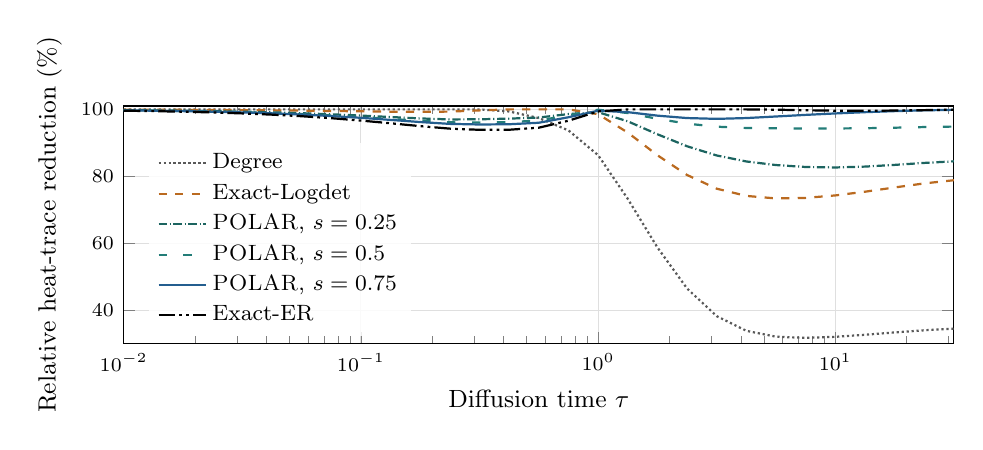
\begin{tikzpicture}
\begin{axis}[
width=\columnwidth,height=4.6cm,
xmode=log,log basis x=10,xmin=.01,xmax=31.6,ymin=30,ymax=101,
xlabel={Diffusion time $\tau$},
ylabel={Relative heat-trace reduction (\%)},
grid=major,major grid style={gray!25},
tick label style={font=\scriptsize},label style={font=\small},
legend pos=south west,legend cell align=left,
legend style={font=\footnotesize,draw=none,fill=white,fill opacity=.85,text opacity=1},
]
\addplot[black!65,densely dotted,line width=.8pt] coordinates {(0.01,100.00) (0.01334,100.00) (0.01778,100.00) (0.02371,100.00) (0.03162,100.00) (0.04217,100.00) (0.05623,100.00) (0.07499,100.00) (0.1,100.00) (0.1334,100.00) (0.1778,100.00) (0.2371,100.00) (0.3162,100.00) (0.4217,99.38) (0.5623,97.41) (0.7499,93.72) (1,86.32) (1.334,73.26) (1.778,58.76) (2.371,46.49) (3.162,38.23) (4.217,33.85) (5.623,32.09) (7.499,31.74) (10,32.06) (13.34,32.67) (17.78,33.37) (23.71,34.01) (31.62,34.50)};
\addlegendentry{Degree}
\addplot[PolarOrange,dashed,line width=.8pt] coordinates {(0.01,99.93) (0.01334,99.90) (0.01778,99.87) (0.02371,99.83) (0.03162,99.78) (0.04217,99.71) (0.05623,99.63) (0.07499,99.53) (0.1,99.42) (0.1334,99.32) (0.1778,99.27) (0.2371,99.34) (0.3162,99.70) (0.4217,100.00) (0.5623,100.00) (0.7499,100.00) (1,98.57) (1.334,93.06) (1.778,86.31) (2.371,80.40) (3.162,76.31) (4.217,74.15) (5.623,73.40) (7.499,73.56) (10,74.30) (13.34,75.41) (17.78,76.68) (23.71,77.89) (31.62,78.84)};
\addlegendentry{Exact-Logdet}
\addplot[PolarTeal!80!black,densely dashdotted,line width=.8pt] coordinates {(0.01,99.78) (0.01334,99.71) (0.01778,99.61) (0.02371,99.49) (0.03162,99.33) (0.04217,99.12) (0.05623,98.86) (0.07499,98.53) (0.1,98.15) (0.1334,97.72) (0.1778,97.30) (0.2371,97.00) (0.3162,97.04) (0.4217,97.24) (0.5623,97.57) (0.7499,98.60) (1,99.16) (1.334,96.43) (1.778,92.57) (2.371,88.98) (3.162,86.23) (4.217,84.44) (5.623,83.37) (7.499,82.79) (10,82.65) (13.34,82.91) (17.78,83.42) (23.71,84.01) (31.62,84.49)};
\addlegendentry{\POLAR{}, $s=0.25$}
\addplot[PolarTeal,loosely dashed,line width=.8pt] coordinates {(0.01,99.73) (0.01334,99.64) (0.01778,99.52) (0.02371,99.37) (0.03162,99.17) (0.04217,98.92) (0.05623,98.59) (0.07499,98.19) (0.1,97.70) (0.1334,97.15) (0.1778,96.59) (0.2371,96.14) (0.3162,96.05) (0.4217,96.20) (0.5623,96.67) (0.7499,98.23) (1,99.90) (1.334,98.91) (1.778,97.19) (2.371,95.74) (3.162,94.83) (4.217,94.45) (5.623,94.34) (7.499,94.29) (10,94.30) (13.34,94.37) (17.78,94.53) (23.71,94.72) (31.62,94.87)};
\addlegendentry{\POLAR{}, $s=0.5$}
\addplot[PolarBlue,solid,line width=.8pt] coordinates {(0.01,99.70) (0.01334,99.61) (0.01778,99.48) (0.02371,99.31) (0.03162,99.10) (0.04217,98.82) (0.05623,98.46) (0.07499,98.01) (0.1,97.48) (0.1334,96.86) (0.1778,96.22) (0.2371,95.67) (0.3162,95.49) (0.4217,95.56) (0.5623,96.01) (0.7499,97.65) (1,99.62) (1.334,99.17) (1.778,98.13) (2.371,97.41) (3.162,97.17) (4.217,97.41) (5.623,97.88) (7.499,98.36) (10,98.79) (13.34,99.17) (17.78,99.48) (23.71,99.72) (31.62,99.87)};
\addlegendentry{\POLAR{}, $s=0.75$}
\addplot[black,dash pattern=on 6pt off 1.5pt on 1pt off 1.5pt on 1pt off 1.5pt,line width=.8pt] coordinates {(0.01,99.61) (0.01334,99.48) (0.01778,99.31) (0.02371,99.09) (0.03162,98.80) (0.04217,98.43) (0.05623,97.96) (0.07499,97.37) (0.1,96.66) (0.1334,95.85) (0.1778,95.00) (0.2371,94.25) (0.3162,93.90) (0.4217,93.92) (0.5623,94.53) (0.7499,96.62) (1,99.39) (1.334,100.00) (1.778,100.00) (2.371,100.00) (3.162,100.00) (4.217,100.00) (5.623,99.91) (7.499,99.74) (10,99.61) (13.34,99.57) (17.78,99.65) (23.71,99.78) (31.62,99.90)};
\addlegendentry{Exact-ER}
\end{axis}
\end{tikzpicture}
\caption{Heat-trace reduction on ca-HepPh (uniform candidate pool,
$k=20$, $\sigma=1$), normalized at each diffusion time by the
largest reduction among the compared selections, rather than
the global optimum. \POLAR{} at $s=0.5$ selects the same edge
set as exact fractional greedy at that exponent. The vertical
axis starts at $30\%$.}
\label{fig:heat}
\end{figure}

On ca-HepPh at $\tau\approx3.2$, Exact-ER gives the largest reduction among
the compared selections; Degree, Exact-Logdet, and \POLAR{} at
$s=0.25,0.5,0.75$ achieve $38.2\%$, $76.3\%$, and $86.2\%$, $94.8\%$,
$97.2\%$ of that observed maximum, respectively. Across the evaluated
uniform pools, Degree leads at the shortest measured times and
inverse-trace selection at the longest, with fractional selections
ordered by $s$ in these tests. On 2-hop pools, ratios for $\tau\ge30$
become rounding-sensitive as the reductions approach zero.

\begin{table}[t]
\centering
\caption{Heat-trace reduction (\%) from saved uniform-pool selections
($\sigma=1$, $M=2000$, $k=20$, $\dsk=128$, $B=16$).
Each row is normalized by the best of Degree, Exact-Logdet,
Exact-ER, and the three \POLAR{} settings, not by a global optimum.
The Degree/Exact-Logdet winners are identified in the text.}
\label{tab:heat-two-horizons}
\footnotesize
\begin{tabular}{@{}lcrrrr@{}}
\toprule
Network & $\tau$ & \multicolumn{3}{c}{\POLAR{} exponent $s$} & Exact-ER\\
\cmidrule(lr){3-5}
 & & $.25$ & $.5$ & $.75$ &\\
\midrule
Hamster & 0.1 & 99.94 & 99.94 & 99.71 & 99.50\\
 & 10 & 96.04 & 96.38 & 97.92 & 100.00\\
email-Eu-core & 0.1 & 90.53 & 88.03 & 81.64 & 81.65\\
 & 10 & 99.99 & 99.99 & 100.00 & 99.75\\
ca-GrQc & 0.1 & 100.00 & 100.00 & 99.10 & 99.33\\
 & 10 & 94.06 & 95.02 & 100.00 & 99.25\\
\bottomrule
\end{tabular}
\end{table}

Table~\ref{tab:heat-two-horizons} extends the comparison to three
networks using their saved heat curves. At $\tau=0.1$, Degree leads
on Hamster and email-Eu-core, while Exact-Logdet leads on ca-GrQc
(the top three entries round to $100\%$). At $\tau=10$, Exact-ER
leads on Hamster and \POLAR{} at $s=0.75$ leads on the other two.
The preferred observed selection depends on both graph and horizon.

\subsection{Parameters and Robustness}
\label{sec:exp-params}

Table~\ref{tab:params} studies $\dsk,B,\epsilon$ on ca-GrQc at $s=0.5$.
Increasing $B$ to 32 matches exact fractional greedy, while larger $\dsk$
generally improves recovery but not monotonically. Tightening $\epsilon$
from $10^{-1}$ to $10^{-4}$ leaves gains unchanged to four decimals
while increasing $q$ from 60 to 110. 

\begin{table}[!t]
\centering
\caption{One-at-a-time parameter sensitivity on ca-GrQc with uniform
candidates ($s=0.5$, $\sigma=1$, $k=20$, $M=2000$). Ratio denotes
the final $f_s$ gain relative to exact fractional greedy. Unless
varied, $\dsk=128$, $B=16$, and $\epsilon=10^{-2}$; pole count $q$
is reported for the tolerance sweep.}
\label{tab:params}
\footnotesize
\setlength{\tabcolsep}{3.4pt}
\renewcommand{\arraystretch}{1.05}
\begin{tabular}{@{}lrrrrrrr@{}}
\toprule
$\dsk$ & 16 & 32 & 64 & 96 & 128 & 192 & 256\\
Ratio & 0.9694 & 0.9801 & 0.9761 & 0.9934 & 0.9952 & 0.9999 & 0.9987\\
Time (s) & 1.64 & 1.66 & 1.83 & 1.95 & 2.17 & 2.48 & 2.64\\
\midrule
$B$ & 1 & 2 & 4 & 8 & 16 & 32 & 64\\
Ratio & 0.9796 & 0.9809 & 0.9826 & 0.9952 & 0.9952 & 1.0000 & 1.0000\\
Time (s) & 1.35 & 1.79 & 1.99 & 2.15 & 2.17 & 2.23 & 3.33\\
\midrule
$\epsilon$ & $10^{-1}$ & $10^{-2}$ & $10^{-3}$ & $10^{-4}$ & & &\\
$q$ & 60 & 80 & 90 & 110 & & &\\
Ratio & 0.9952 & 0.9952 & 0.9952 & 0.9952 & & &\\
Time (s) & 2.02 & 2.17 & 2.24 & 2.44 & & &\\
\bottomrule
\end{tabular}
\end{table}

\paragraph{Sketch construction}
We test sensitivity to the sketch distribution and size. Across five seeds on three medium networks, block-orthogonal sketches
at $\dsk=128,B=16$ achieve mean ratios of $0.9938$--$0.9997$, versus
$0.9887$--$0.9997$ for Gaussian sketches. Reducing to $\dsk=24,B=4$ lowers
block-orthogonal recovery to $0.9480$--$0.9909$, although the same small
configuration is stable on the controlled multiscale benchmark.

\paragraph{Per-round recovery and error attribution}
We estimate per-round recovery $r_i$ (the selected marginal divided by
the largest available marginal) using dense eigendecomposition and
quadrature with relative target $10^{-9}$ to score all candidates along
each recorded trajectory. With default parameters, trajectory means are
$0.964$--$1.000$ and minima are $0.900$--$1.000$; $58$--$96\%$ of rounds
attain the reference maximum within $10^{-8}$ relative tolerance.
These statistics are neither final-gain ratios nor the certificates of
Lemma~\ref{lem:approximate-greedy} (Remark~\ref{rem:average-beta} in
Section~\ref{sec:numerical-errors}).

To locate selection loss, we compare the selected and shortlist-best
reference marginals, each normalized by the global reference maximum.
Across Hamster, ca-GrQc, and email-Eu-core, we test block-orthogonal
sketches at $(\dsk,B)=(24,4),(128,16)$ and Gaussian sketches at
$(128,16)$, with five seeds and 20 rounds each: 900 decisions in total.
The two normalized scores differ by at most $1.8\times10^{-15}$.
Thus the observed per-round loss arises from shortlist omissions, not
from re-ranking within the shortlist.

\paragraph{Candidate pools, budget, and regularization}
These checks vary the default workload. Across three independently sampled uniform pools on each of three
medium networks, \POLAR{} recovers $0.9889$--$1.0000$ of exact greedy.
With $k=100$ on the ca-GrQc 2-hop pool, its $s=0.5$ ratio is $0.9929$,
versus $0.9793$ for Exact-ER, $0.9918$ for Degree, and $0.9988$ for
Exact-Logdet. On the default $k=20$ uniform pools, \POLAR{} matches
exact fractional greedy at $s=0.5$ for $\sigma\in\{0.01,0.1\}$; at
$\sigma=0.01$, its Jaccard similarity to Exact-ER is $0.74$--$1.00$,
while Degree attains only $0.20$--$0.58$ of the best reported $f_{0.5}$
gain. 

\paragraph{Limitations}
We measure spectral gains, selected-edge structure, and heat-trace
responses, not downstream benefits in deployed graph-management
applications. Principal runtime
measurements fix $\sigma=1$, $M=2000$, and $k=20$; the quality
checks at smaller $\sigma$ or larger $k$ do not establish runtime
scaling in those regimes. Smaller $\sigma$ worsens the unpreconditioned
CG bound. Preconditioning or SDD solve
backends~\cite{spielman2014solver,koutis2011,kyng2016}, with shift
sharing accounted for, remain future work. The common-affine heap
has no performance evaluation.

\section{Related Work}
\label{sec:related}

\paragraph{Spectral objectives and graph modification}
Effective-resistance design and discrete edge augmentation prioritize
global connectivity~\cite{ghosh2008,predari2023}, while current-flow
group measures~\cite{li2019group,xia2025current}, forest-matrix
proximity~\cite{sun2024forest,grinten2021forest}, opinion
optimization~\cite{sun2025opinion}, and Kemeny's
constant~\cite{li2021kemeny,kirkland2025} motivate other spectral
quantities. FastFrac~\cite{fastfrac}
optimizes the submodular positive-power side of the log-determinant,
where increasing $s$ flattens the mode weights; here it steepens them
toward low frequencies.

Experimental design studies related spectral criteria for
measurement selection through
approximate supermodularity~\cite{chamon2017} and proportional
volume sampling~\cite{nikolov2019}. Arrigo and Benzi~\cite{arrigo2016} instead optimize
network communicability based on adjacency-matrix exponentials.

\paragraph{Marginal estimation and computational reuse}
Contour quadrature~\cite{hale2008} and rational Krylov
methods~\cite{benzi2022} evaluate matrix functions; SLQ estimates
traces~\cite{ubaru2017}, with numerical analyses in~\cite{musco2018,chen2022}.
Edge selection needs relative accuracy for small rank-one trace changes,
which separate trace estimates need not provide. Shifted Krylov
methods~\cite{jegerlehner1996,frommer1998} share iterations across poles;
SDD solvers~\cite{spielman2014solver,koutis2011}, sparse
elimination~\cite{kyng2016}, and sparsification~\cite{spielman2011,batson2012}
provide complementary primitives. General low-rank matrix-function
updates~\cite{beckermann2018} and rational Krylov
extensions~\cite{beckermann2021} already enable reuse.
\POLAR{} specializes to fractional edge marginals, sharing shifted
solves and maintained quantities across many candidates and rounds.

\paragraph{Greedy selection and fixed sketches}
Classical lazy greedy relies on diminishing returns~\cite{leskovec2007};
ratio--curvature analysis~\cite{bian2017} handles non-submodular
objectives. We specialize the latter to fractional gains and combine
it with numerical errors. Fixed-sketch projection
bounds~\cite{skorski2021} and lossless proxy ranking address distinct
accuracy requirements.

\section{Conclusion}
\label{sec:conclusion}
\POLAR{} combines relative-accuracy quadrature, shared solves, and
cross-round reuse for fractional inverse-trace selection. Conditional
guarantees and experiments distinguish similar-value, different-edge
regimes from controlled competition with larger value gaps.
Separate heat responses show that different diffusion horizons
favor different selections.

\section*{Acknowledgment}
Generative AI tools, including OpenAI ChatGPT/Codex and Anthropic
Claude, assisted with language editing and code implementation.
They also helped develop parts of the proofs and identify
counterexamples based on the authors' ideas and preliminary
verification approaches. The authors reviewed the AI-assisted
content, checked its accuracy, and take full responsibility
for the final manuscript.



\begin{thebibliography}{36}

\bibitem{ghosh2008}
A.~Ghosh, S.~Boyd, and A.~Saberi,
``Minimizing effective resistance of a graph,''
\emph{SIAM Review}, vol.~50, no.~1,
pp.~37--66, 2008, doi: 10.1137/050645452.

\bibitem{predari2023}
M.~Predari, L.~Berner, R.~Kooij, and H.~Meyerhenke,
\lq\lq{}Greedy optimization of resistance-based graph robustness with global and local edge insertions,''
\emph{Social Network Analysis and Mining}, vol.~13, Art.~130, 2023,
doi: 10.1007/s13278-023-01137-1.

\bibitem{black2023}
M.~Black, Z.~Wan, A.~Nayyeri, and Y.~Wang,
``Understanding oversquashing in GNNs through the lens of effective resistance,''
in \emph{Proc. ICML}, PMLR, vol.~202, 2023, pp.~2528--2547.

\bibitem{kirkland2025}
S.~Kirkland, Y.~Li, J.~S.~McAlister, and X.~Zhang,
``Edge addition and the change in Kemeny's constant,''
\emph{Discrete Applied Mathematics}, vol.~373,
pp.~77--90, 2025, doi: 10.1016/j.dam.2025.04.031.

\bibitem{fastfrac}
``FastFrac: Fast edge recommendation for fractional spectral traces
on graphs,'' companion submission to \emph{IEEE ICDE}, 2027. [Online]. Available:
\url{https://github.com/chenty2333/POLAR/blob/main/paper/FastFrac.pdf}

\bibitem{leskovec2007}
J.~Leskovec, A.~Krause, C.~Guestrin, C.~Faloutsos,
J.~VanBriesen, and N.~Glance,
\lq\lq{}Cost-effective outbreak detection in networks,''
in \emph{Proc. ACM SIGKDD}, 2007, pp.~420--429.

\bibitem{jegerlehner1996}
B.~Jegerlehner,
\lq\lq{}Krylov space solvers for shifted linear systems,''
arXiv:hep-lat/9612014, 1996.

\bibitem{bian2017}
A.~A.~Bian, J.~M.~Buhmann, A.~Krause, and S.~Tschiatschek,
\lq\lq{}Guarantees for greedy maximization of non-submodular functions with applications,''
in \emph{Proc. ICML}, PMLR, vol.~70, pp.~498--507, 2017.

\bibitem{dlmf-quadrature}
NIST, \emph{Digital Library of Mathematical Functions},
Sec.~3.5, \lq\lq{}Quadrature.''
[Online]. Available: \url{https://dlmf.nist.gov/3.5}

\bibitem{dlmf-jacobi}
NIST, \emph{Digital Library of Mathematical Functions},
Sec.~18.3, \lq\lq{}Definitions.''
[Online]. Available: \url{https://dlmf.nist.gov/18.3}

\bibitem{spielman2011}
D.~A.~Spielman and N.~Srivastava,
\lq\lq{}Graph sparsification by effective resistances,''
\emph{SIAM Journal on Computing}, vol.~40, no.~6,
pp.~1913--1926, 2011, doi: 10.1137/080734029.

\bibitem{skorski2021}
M.~Skorski,
\lq\lq{}Johnson--Lindenstrauss transforms with best confidence,''
in \emph{Proc. COLT}, PMLR, vol.~134, pp.~3989--4007, 2021.

\bibitem{konect}
J.~Kunegis,
``KONECT: The Koblenz network collection,''
in \emph{Proc. WWW Companion}, 2013, pp.~1343--1350,
doi: 10.1145/2487788.2488173.

\bibitem{snap}
J.~Leskovec and A.~Krevl,
``SNAP Datasets: Stanford large network dataset collection,''
June 2014. [Online]. Available: \url{https://snap.stanford.edu/data/}

\bibitem{ubaru2017}
S.~Ubaru, J.~Chen, and Y.~Saad,
``Fast estimation of $\mathrm{tr}(f(A))$ via stochastic Lanczos quadrature,''
\emph{SIAM Journal on Matrix Analysis and Applications}, vol.~38, no.~4,
pp.~1075--1099, 2017, doi: 10.1137/16M1104974.

\bibitem{polar-repo}
\POLAR{}: Code, data, and experimental results. [Online]. Available: \url{https://github.com/chenty2333/POLAR}

\bibitem{spielman2014solver}
D.~A.~Spielman and S.-H.~Teng,
``Nearly linear time algorithms for preconditioning and solving symmetric, diagonally dominant linear systems,''
\emph{SIAM Journal on Matrix Analysis and Applications}, vol.~35, no.~3,
pp.~835--885, 2014, doi: 10.1137/090771430.

\bibitem{koutis2011}
I.~Koutis, G.~L.~Miller, and R.~Peng,
``A nearly-$m\log n$ time solver for SDD linear systems,''
in \emph{Proc. IEEE FOCS}, 2011, pp.~590--598,
doi: 10.1109/FOCS.2011.85.

\bibitem{kyng2016}
R.~Kyng and S.~Sachdeva,
``Approximate Gaussian elimination for Laplacians---fast, sparse, and simple,''
in \emph{Proc. IEEE FOCS}, 2016, pp.~573--582,
doi: 10.1109/FOCS.2016.68.

\bibitem{li2019group}
H.~Li, R.~Peng, L.~Shan, Y.~Yi, and Z.~Zhang,
``Current flow group closeness centrality for complex networks,''
in \emph{Proc. The Web Conference (WWW)}, 2019,
pp.~961--971, doi: 10.1145/3308558.3313490.

\bibitem{xia2025current}
H.~Xia and Z.~Zhang,
``Fast maximization of current flow group closeness centrality,''
in \emph{Proc. IEEE ICDE}, 2025,
doi: 10.1109/ICDE65448.2025.00241.

\bibitem{sun2024forest}
H.~Sun, X.~Zhou, and Z.~Zhang,
``Fast computation for the forest matrix of an evolving graph,''
in \emph{Proc. ACM SIGKDD}, 2024, pp.~2755--2764,
doi: 10.1145/3637528.3671822.

\bibitem{grinten2021forest}
A.~van der Grinten, E.~Angriman, M.~Predari, and H.~Meyerhenke,
``New approximation algorithms for forest closeness centrality---for individual vertices and vertex groups,''
in \emph{Proc. SIAM SDM}, 2021, pp.~136--144,
doi: 10.1137/1.9781611976700.16.

\bibitem{sun2025opinion}
H.~Sun, Y.~Sun, X.~Zhou, and Z.~Zhang,
``Fast computation and optimization for opinion-based quantities of Friedkin--Johnsen model,''
in \emph{Advances in Neural Information Processing Systems}, vol.~38, 2025,
doi: 10.52202/085713-1269.

\bibitem{li2021kemeny}
S.~Li, X.~Huang, and C.-H.~Lee,
``An efficient and scalable algorithm for estimating Kemeny's constant of a Markov chain on large graphs,''
in \emph{Proc. ACM SIGKDD}, 2021, pp.~964--974,
doi: 10.1145/3447548.3467431.

\bibitem{chamon2017}
L.~F.~O.~Chamon and A.~Ribeiro,
``Approximate supermodularity bounds for experimental design,''
in \emph{Advances in Neural Information Processing Systems},
vol.~30, 2017, pp.~5403--5412.

\bibitem{nikolov2019}
A.~Nikolov, M.~Singh, and U.~T.~Tantipongpipat,
``Proportional volume sampling and approximation algorithms for
A-optimal design,'' in \emph{Proc. ACM--SIAM SODA}, 2019,
pp.~1369--1386, doi: 10.1137/1.9781611975482.84.

\bibitem{arrigo2016}
F.~Arrigo and M.~Benzi,
``Updating and downdating techniques for optimizing network
communicability,'' \emph{SIAM Journal on Scientific Computing},
vol.~38, no.~1, pp.~B25--B49, 2016, doi: 10.1137/140991923.

\bibitem{hale2008}
N.~Hale, N.~J.~Higham, and L.~N.~Trefethen,
``Computing $A^\alpha$, $\log(A)$ and related matrix functions by contour integrals,''
\emph{SIAM Journal on Numerical Analysis}, vol.~46, no.~5,
pp.~2505--2523, 2008, doi: 10.1137/070700607.

\bibitem{benzi2022}
M.~Benzi and I.~Simunec,
\lq\lq{}Rational Krylov methods for fractional diffusion problems on graphs,''
\emph{BIT Numerical Mathematics}, vol.~62, pp.~357--385, 2022,
doi: 10.1007/s10543-021-00881-0.

\bibitem{musco2018}
C.~Musco, C.~Musco, and A.~Sidford,
``Stability of the Lanczos method for matrix function approximation,''
in \emph{Proc. ACM--SIAM SODA}, 2018, pp.~1605--1624,
doi: 10.1137/1.9781611975031.105.

\bibitem{chen2022}
T.~Chen, A.~Greenbaum, C.~Musco, and C.~Musco,
``Error bounds for Lanczos-based matrix function approximation,''
\emph{SIAM Journal on Matrix Analysis and Applications}, vol.~43, no.~2,
pp.~787--811, 2022, doi: 10.1137/21M1427784.

\bibitem{frommer1998}
A.~Frommer and U.~Gl\"assner,
``Restarted GMRES for shifted linear systems,''
\emph{SIAM Journal on Scientific Computing}, vol.~19, no.~1,
pp.~15--26, 1998, doi: 10.1137/S1064827596304563.

\bibitem{batson2012}
J.~Batson, D.~A.~Spielman, and N.~Srivastava,
``Twice-Ramanujan sparsifiers,''
\emph{SIAM Journal on Computing}, vol.~41, no.~6,
pp.~1704--1721, 2012, doi: 10.1137/090772873.

\bibitem{beckermann2018}
B.~Beckermann, D.~Kressner, and M.~Schweitzer,
``Low-rank updates of matrix functions,''
\emph{SIAM Journal on Matrix Analysis and Applications},
vol.~39, no.~1, pp.~539--565, 2018, doi: 10.1137/17M1140108.

\bibitem{beckermann2021}
B.~Beckermann, A.~Cortinovis, D.~Kressner, and M.~Schweitzer,
``Low-rank updates of matrix functions II: Rational Krylov methods,''
\emph{SIAM Journal on Numerical Analysis},
vol.~59, no.~3, pp.~1325--1347, 2021, doi: 10.1137/20M1362553.

\end{thebibliography}
\end{document}

